\chapter{保护}
\section{引言}
保护是五大关键设计和运行项目之一——其他四项是稳定性、机械完整性、制冷和导体。




\subsection{热能密度 vs. 磁能密度}
除非绕组得到了保护,不然磁体绕组的一小部分,即“热点”,就要吸收掉存储于绕组中的大部分磁能。这样,该部分将过热并永久性损坏。
不过,熔化磁体中单位绕组体积的热能密度要远大于磁体存储的磁能密度。

仅考虑将磁体内部空间内存储的能量全部绝热转换为热,引起铜(绕组的一种代表性材料)的焓密度$h_{Cu}(T)$变化。如果是从4K(或者80K)加热到它的熔点1356K,
那么初始磁感应密度$B_0$将高达$~150 T$:
\begin{equation}% 8.1第一个
\frac{B_{0}^{2}}{2\mu_o}=h_{cu}(1356\ \mathrm{K})-h_{cu}(4\ \mathrm{K}\ \mathrm{or}80\ \mathrm{K})\simeq 5.2\times 10^9\ \mathrm{J/m^3}
\end{equation}
\begin{equation}% 8.1第二个
B_0\simeq\sqrt{2(4\pi\times 10^{-7}\ \mathrm{H/m})(5.2\times 10^9\ \mathrm{J/m^3})}\simeq 115\ \mathrm{T}
\end{equation}

\subsection{热点和热点温度}

\begin{equation}% page468 3.79
E_m=\frac{1}{2}LI^2
\end{equation}
\begin{equation}% page468 3.81
L=\mu_oa_1\ \mathcal{L}(\alpha,\beta)N^2
\end{equation}
\begin{equation}% 8.2
B_o=\frac{\mu_oNI}{2a_1(\alpha-1)\beta}F(\alpha,\beta)
\end{equation}
\begin{equation}% page468 3.13b
F(\alpha,\beta)=\beta\left(\frac{\alpha+\sqrt{\alpha^2+\beta^2}}{1+\sqrt{1+\beta^2}}\right)
\end{equation}
\begin{equation}% 8.3
NI=\frac{2a_1(\alpha-1)\beta B_o}{\mu_oF(\alpha,\beta)}
\end{equation}
\begin{equation}% 8.4
E_m=\frac{4a_{1}^{3}(\alpha-1)^2\beta^2\ \mathcal{L}(\alpha,\beta)}{F^2(\alpha,\beta)}\left(\frac{B_{o}^{2}}{2\mu_o}\right)
\end{equation}
\begin{equation}% 8.5
V_w=2\pi a_{1}^{3}(\alpha^2-1)\beta
\end{equation}
\begin{equation}% 8.6
V_r=f_eV_w=f_r2\pi a_{1}^{3}(\alpha^2-1)\beta
\end{equation}
\begin{equation}% 8.7
e_{mr}=\frac{E_m}{V_r}=\frac{2(\alpha-1)\beta\ \mathcal{L}(\alpha,\beta)}{f_r\pi(\alpha+1)F^2(\alpha,\beta)}\left(\frac{B_{o}^{2}}{2\mu_o}\right)
\end{equation}


\subsection{绕组材料的温度数据}



\subsection{安全、风险和高度风险$T_f$区间}


\subsection{温度引起的应变}



\section{绝热加热}

\begin{equation}% 8.8a和8.8b
C_{cd}(T)\frac{dT}{dt}\simeq\rho_{cd}(T)J_{cd_o}^{2}(t) 
\simeq\rho_m(T)J_{cd_o}^{2}(t)
\end{equation}

\subsection{恒定电流模式下的绝热加热}
\begin{equation}% 8.9a
A_{cd}C_{cd}(T)\frac{dT}{dt}=\frac{\rho_m(T)}{A_m}I_{op}^{2}(t)
\end{equation}
\begin{equation}% 8.9b
C_m(T)\frac{dT}{dt}=\left(\frac{A_m}{A_{cd}}\right)\rho_m(T)J_{m_o}^{2}=\left(\frac{\gamma_{m/s}}{1+\gamma_{m/s}}\right)\rho_m(T)J_{m_o}^{2}
\end{equation}
\begin{equation}% 8.9c和8.9d
\int_{T_i}^{T_f}\frac{C_m(T)}{\rho_m(T)}dT=\left(\frac{A_m}{A_{cd}}\right)J_{m_o}^{2}\tau_{ah} 
=\left(\frac{\gamma_{m/s}}{1+\gamma_{m/s}}\right)J_{m_o}^{2}\tau_{ah}
\end{equation}
\begin{equation}% 8.10a
Z(T_f,T_i)\equiv\int_{T_i}^{T_f}\frac{C_m(T)}{\rho_m(T)}dT
\end{equation}
\begin{equation}% 8.10b
Z(T_f,T_i)\simeq\frac{1}{\tilde{\rho}_m}\int_{T_i}^{T_f}C_m(T_f)dT=\frac{H_m(T_f)-H_m(T_i)}{\tilde{\rho}_m}
\end{equation}


\begin{figure}
	\centering
	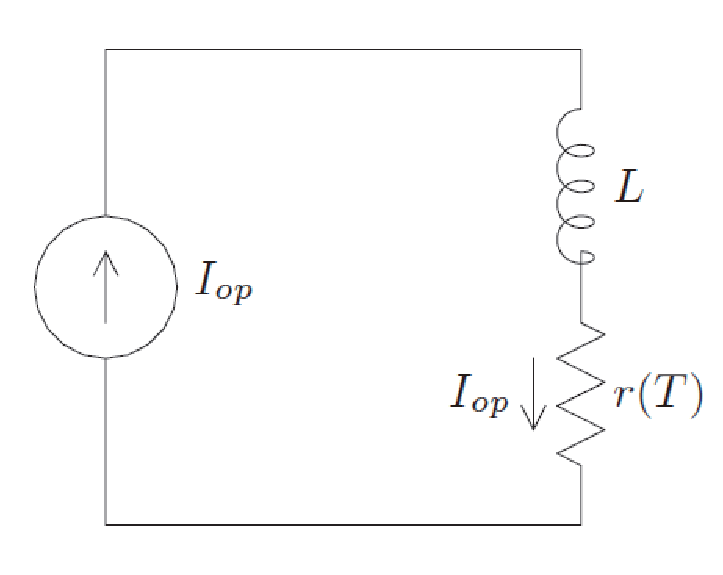
\includegraphics[scale=0.6]{chpt8/figs/fig8.1.eps}
	\caption{Circuit representing a superconducting magnet of inductance L with a normal
		zone of T-dependent resistance r(T), connected to a supply of constant-current Iop..}
\end{figure}


\begin{equation}% 8.11
Z(T_f,T_i)=Z(T_f,0)-Z(T_i,0)=Z(T_f)-Z(T_i)
\end{equation}
\begin{equation}% 8.12a
\tau_{ah}^{i}(T_f,T_i)=\left(\frac{1+\gamma_{m/s}}{\gamma_{m/s}}\right)\frac{Z(T_f,T_i)}{J_{m_o}^{2}}
\end{equation}
\begin{equation}% 8.12b
J_{m_o}^{i}(T_f,T_i)=\sqrt{\left(\frac{1+\gamma_{m/s}}{\gamma_{m/s}}\right)\frac{Z(T_f,T_i)}{\tau_{ah}}}
\end{equation}


\begin{figure}
	\centering
	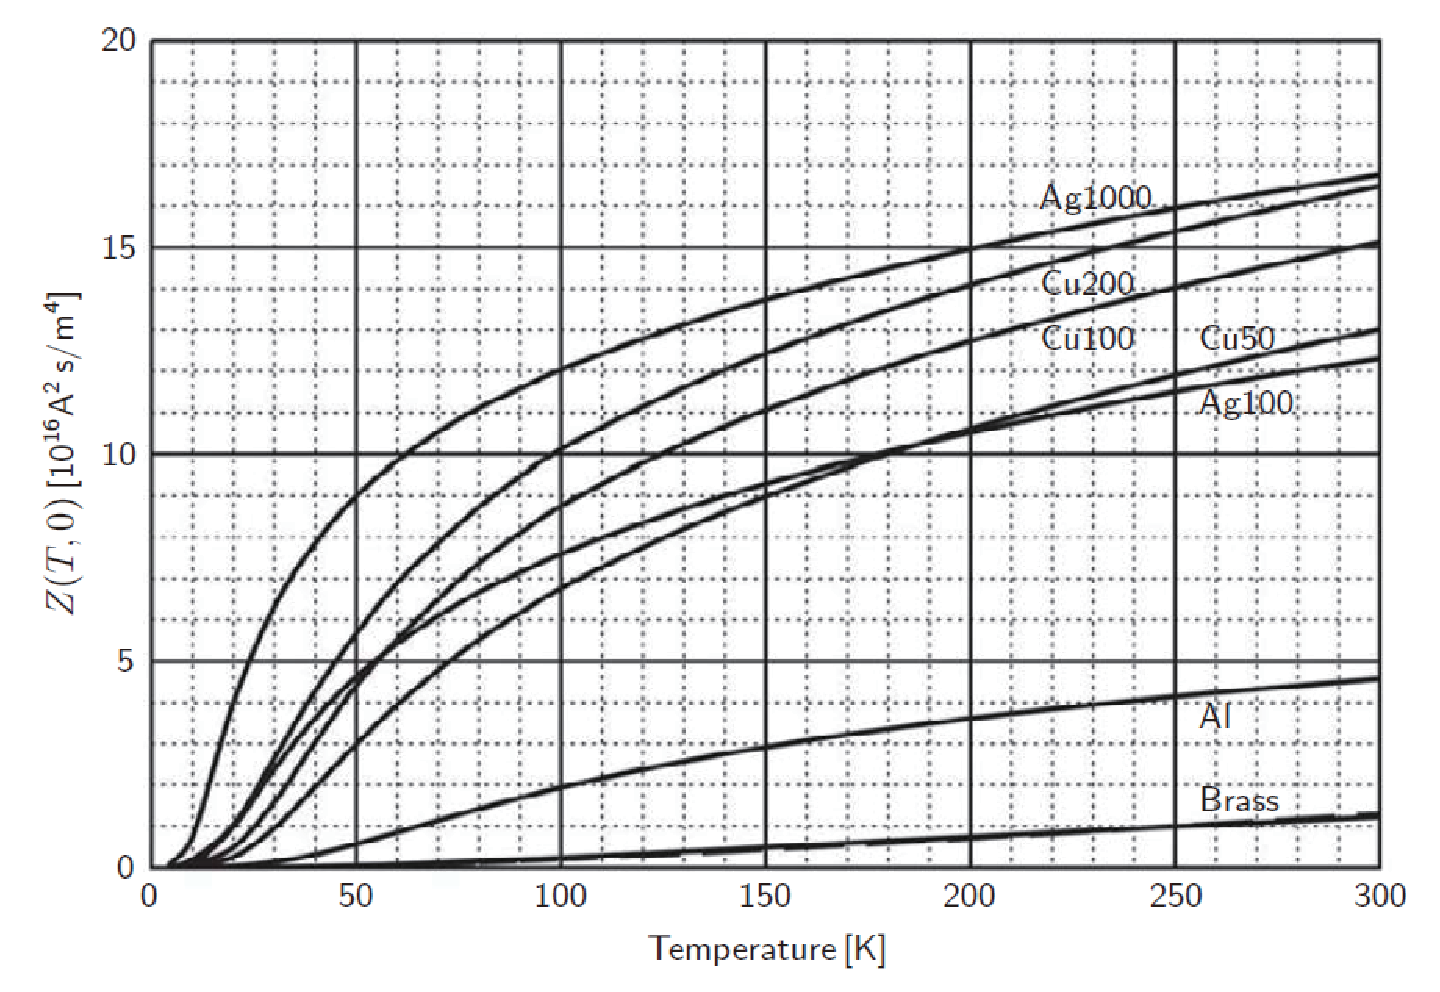
\includegraphics[scale=0.6]{chpt8/figs/fig8.2.eps}
	\caption{Z(T, 0) plots. .}
\end{figure}

\subsection{恒定放电模式下的绝热加热}

\begin{equation}% 8.13
C_m(T)\frac{dT}{dt}=\left(\frac{A_m}{A_{cd}}\right)\rho_m(T)J_{m}^{2}(t)
\end{equation}

\begin{equation}% 8.14
L\frac{dI_m(t)}{dt}+[R_D+r(t)]I_m(t)=0
\end{equation}

\begin{equation}% 8.15
J_m(t)=J_{m_o}e^{-t/\tau_{dg}}
\end{equation}


\begin{subequations}% 8.16a 8.16b 8.16c
	\begin{align*}
Z(T_f,T_i)&=\left(\frac{A_m}{A_{cd}}\right)\int_{0}^{\infty}J_{m_o}^{2}e^{-2t/\tau_{dg}}dt=\left(\frac{A_m}{A_{cd}}\right)J_{m_o}^{2}\times\frac{1}{2}\tau_{dg} \\
&=\left(\frac{A_m}{A_{cd}}\right)J_{m_o}^{2}\left(\frac{L}{2R_D}\right)\\ 
&=\left(\frac{\gamma_{m/s}}{1+\gamma_{m/s}}\right)J_{m_o}^{2}\left(\frac{L}{2R_D}\right)
\end{align*}
\end{subequations}

\begin{figure}
\centering
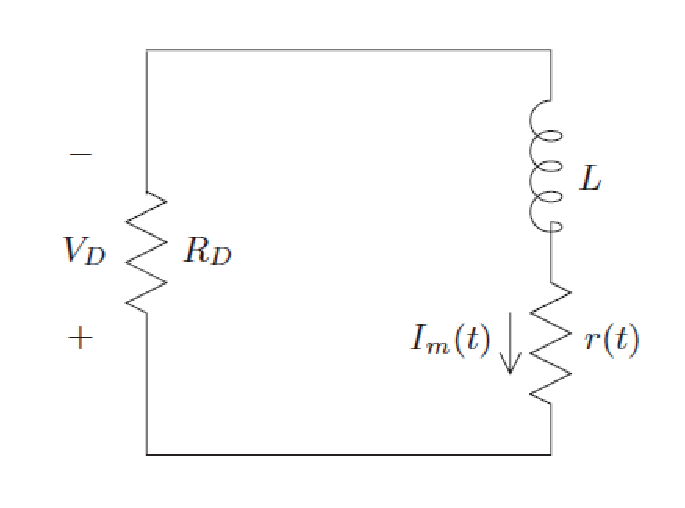
\includegraphics[scale=0.6]{chpt8/figs/fig8.3.eps}
\caption{Circuit representing a superconducting magnet of inductance L.}
\end{figure}


\begin{equation}% 8.17a
L=\frac{2E_m}{I_{op}^{2}}
\end{equation}

\begin{equation}% 8.17b
R_D=\frac{V_D}{I_{op}}
\end{equation}

\begin{equation}% 8.18a
Z(T_f,T_i)=\left(\frac{A_m}{A_{cd}}\right)\frac{J_{m_o}^{2}E_m}{V_DI_{op}}
\end{equation}

\begin{equation}% 8.18b
Z(T_f,T_i)=\frac{J_{m_o}^{2}E_m}{A_{cd}V_D}
\end{equation}

\begin{equation}% 8.19
J_{m_o}^{D}=\frac{A_{cd}V_DZ(T_f,T_i)}{E_m}
\end{equation}

\subsection{引线短接的磁体的绝热加热}



\begin{figure}
	\centering
	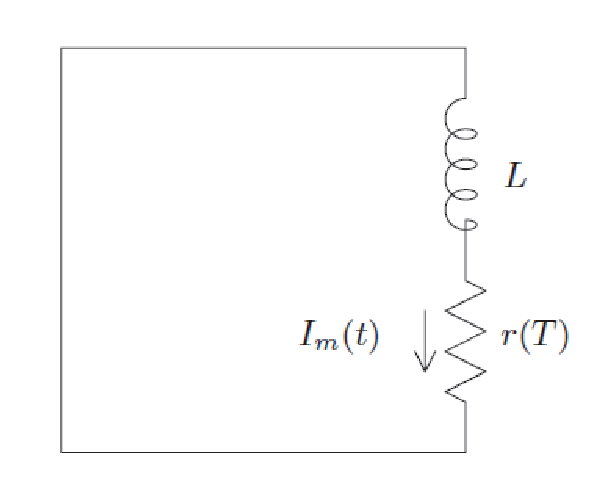
\includegraphics[scale=0.6]{chpt8/figs/fig8.4.eps}
	\caption{Circuit representing a shorted superconducting magnet of inductance.}
\end{figure}

\begin{equation}% 8.20
L\frac{dI_m(t)}{dt}+r(T)I_m(t)=0
\end{equation}

\begin{equation}% 8.21
R_{nz}=\frac{\rho_m(T_f)\ell_{nz}}{4A_m}
\end{equation}

\begin{equation}% 8.22
J_m(t)=J_{m_o}e^{-t/(L/R_{nz})}
\end{equation}


\begin{subequations}% 8.23a,b,c
	\begin{align*}
Z(T_f,T_i)&=\left(\frac{A_m}{A_{cd}}\right)\int_{0}^{\infty}J_{m_o}^{2}e^{-2t/(L/R_{nz})}dt\\
Z(T_f,T_i)&=\frac{1}{2}\left(\frac{A_m}{A_{cd}}\right)J_{m_o}^{2}\left(\frac{L}{R_{nz}}\right) \\
&=\frac{1}{2}\left(\frac{A_m}{A_{cd}}\right)J_{m_o}^{2}\tau_{dg}
\end{align*}
\end{subequations}

\begin{equation}% 8.24
\ell_{nz}=f_r\pi a_1(\alpha+1)N
\end{equation}


\begin{equation}% 8.25
R_{nz}=f_r\frac{\rho_m(T_f)\pi a_1(\alpha+1)N}{4A_m}
\end{equation}


\begin{equation}% 8.26
N=\sqrt{\frac{L}{\mu_oa_1\ \mathcal{L}(\alpha,\beta)}}
\end{equation}


\begin{equation}% 8.27
R_{nz}=f_r\frac{\pi(\alpha+1)\rho_m(T_f)}{4A_m}\sqrt{\frac{a_1L}{\mu_o\ \mathcal{L}(\alpha,\beta)}}
\end{equation}

\begin{subequations}% 8.28a,b
	\begin{align*}
\tau_{dg}&=\frac{L}{R_{nz}}=\frac{4A_m}{f_r\pi(\alpha+1)\rho_m(T_f)}\sqrt{\frac{\mu_o\ \mathcal{L}(\alpha,\beta)L}{a_1}}\\
\tau_{dg}=\frac{4}{f_r\pi(\alpha+1)\rho_m(T_f)J_{m_o}}\sqrt{\frac{2\mu_o\ \mathcal{L}(\alpha,\beta)E_m}{a_1}}
\end{align*}
\end{subequations}

\begin{equation}% 8.29
\rho_m(T_f)Z(T_f,T_i)=\left(\frac{A_m}{A_{cd}}\right)\frac{2J_{m_o}}{f_r\pi(\alpha+1)}\sqrt{\frac{2\mu_o\ \mathcal{L}(\alpha,\beta)E_m}{a_1}}
\end{equation}

\begin{subequations}% 8.30a,b
	\begin{align*}
J_{m_o}^{sh}&=\frac{1}{2}\left(\frac{A_{cd}}{A_m}\right)f_r\pi(\alpha+1)\rho_m(T_f)Z(T_f,T_i)\sqrt{\frac{a_1}{2\mu_o\ \mathcal{L}(\alpha,\beta)E_m}}\\
J_{m_o}^{sh}(T_f,T_i)&=\frac{1}{2}\left(\frac{A_{cd}}{A_m}\right)\frac{f_r\pi(\alpha+1)\rho_m(T_f)Z(T_f,T_i)}{\mu_o\ \mathcal{L}(\alpha,\beta)NI_{op}}
\end{align*}
\end{subequations}


\subsection{恒定电压模式下的绝热加热}

\begin{subequations}% 8.31a,b
	\begin{align*}
A_{cd}\ell_{cd}C_{cd}(T)\frac{dT}{dt}&=\frac{V_{op}^{2}}{R_n(T)}=\frac{V_{op}^{2}A_m}{\rho_m(T)\ell_{cd}}
C_m(T)\frac{dT}{dt}\\\notag
&\simeq\left(\frac{A_m}{A_{cd}}\right)\frac{V_{op}^{2}}{\rho_m(T)\ell_{cd}^{2}}\\
\int_{T_i}^{T_f}C_m(T)\rho_m(T)dT&=\left(\frac{A_m}{A_{cd}}\right)\frac{V_{op}^{2}}{\ell_{cd}^{2}}\tau_{ah}
\end{align*}
\end{subequations}


\begin{subequations}% 8.32a,b,c
	\begin{align*}
Y(T_f,T_i)&\equiv\int_{T_i}^{T_f}C_m(T)\rho_m(T)dT\\
Y(T_f,T_i)&\simeq\tilde{\rho}_m[H_m(T_f)-H_m(T_i)]\\
Y(T_f,T_i)&=Y(T_f)-Y(T_i)
\end{align*}
\end{subequations}



\begin{figure}
	\centering
	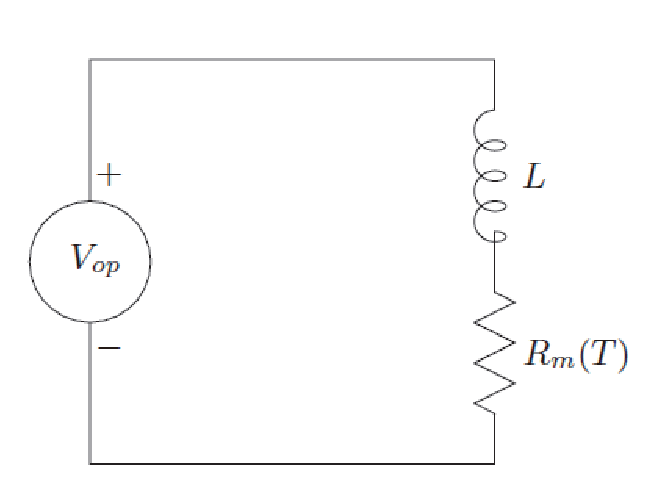
\includegraphics[scale=0.6]{chpt8/figs/fig8.5.eps}
	\caption{Circuit for a superconducting magnet (L) with the entire winding}
\end{figure}


\begin{equation}% 8.33
Y(T_f,T_i)=\left(\frac{A_m}{A_{cd}}\right)\frac{V_{op}^{2}\tau_{ah}}{\ell_{cd}^{2}}
\end{equation}
\begin{equation}% 8.34
\ell_{cd}=\pi(\alpha+1)\sqrt{\frac{a_1L}{\mu_o\ \mathcal{L}(\alpha,\beta)}}
\end{equation}
\begin{equation}% 8.35
Y(T_f,T_i)=\left(\frac{A_m}{A_{cd}}\right)\frac{\mu_o\ \mathcal{L}(\alpha,\beta)V_{op}^{2}\tau_{ah}}{\pi^2(\alpha+1)^2a_1L}
\end{equation}

\begin{equation}% 8.36
\tau_{ah}^{\upsilon}=\left(\frac{A_{cd}}{A_m}\right)\frac{\pi^2(\alpha+1)^2a_1L}{\mu_o\ \mathcal{L}(\alpha,\beta)}\left[\frac{Y(T_f,T_i)}{V_{op}^{2}}\right]
\end{equation}



\begin{figure}
	\centering
	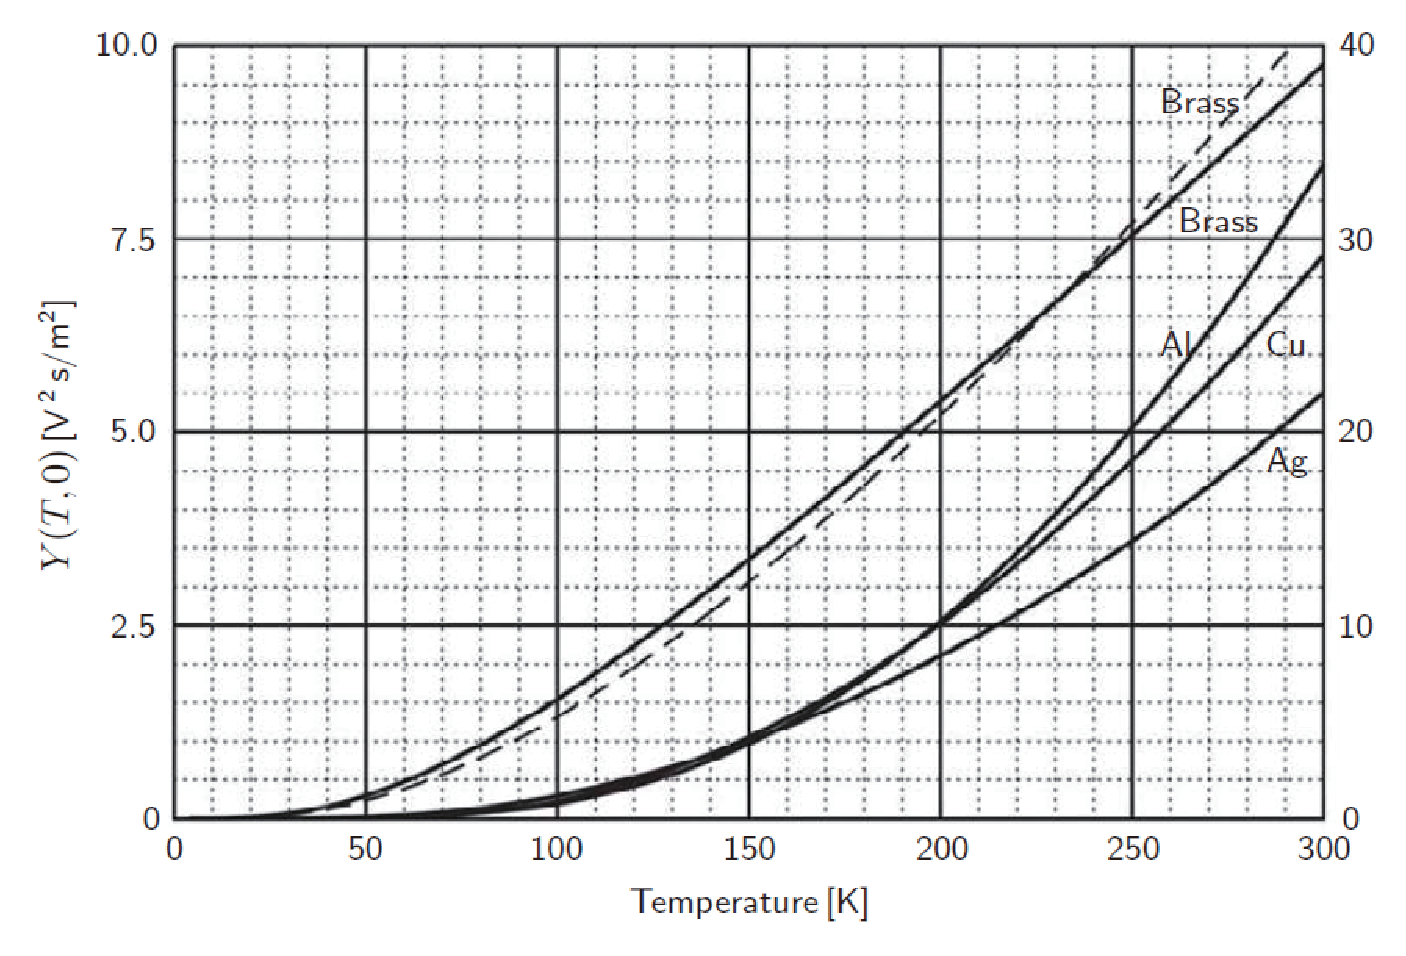
\includegraphics[scale=0.6]{chpt8/figs/fig8.6.eps}
	\caption{Y (T,0) plots. Left-hand vertical scal}
\end{figure}

\section{高电压}


\begin{subequations}% 8.37a,b
	\begin{align*}
V&=L\frac{dI}{dt}\\
V&=\frac{2E_m}{I_{o}^{2}}\left(\frac{\Delta I}{\Delta t}\right)\approx\frac{2E_m}{I_o\Delta t}
	\end{align*}
\end{subequations}



\subsection{电弧环境}

\subsection{Paschen电压试验}

\subsection{失超磁体内的电压峰值}



\begin{figure}
	\centering
	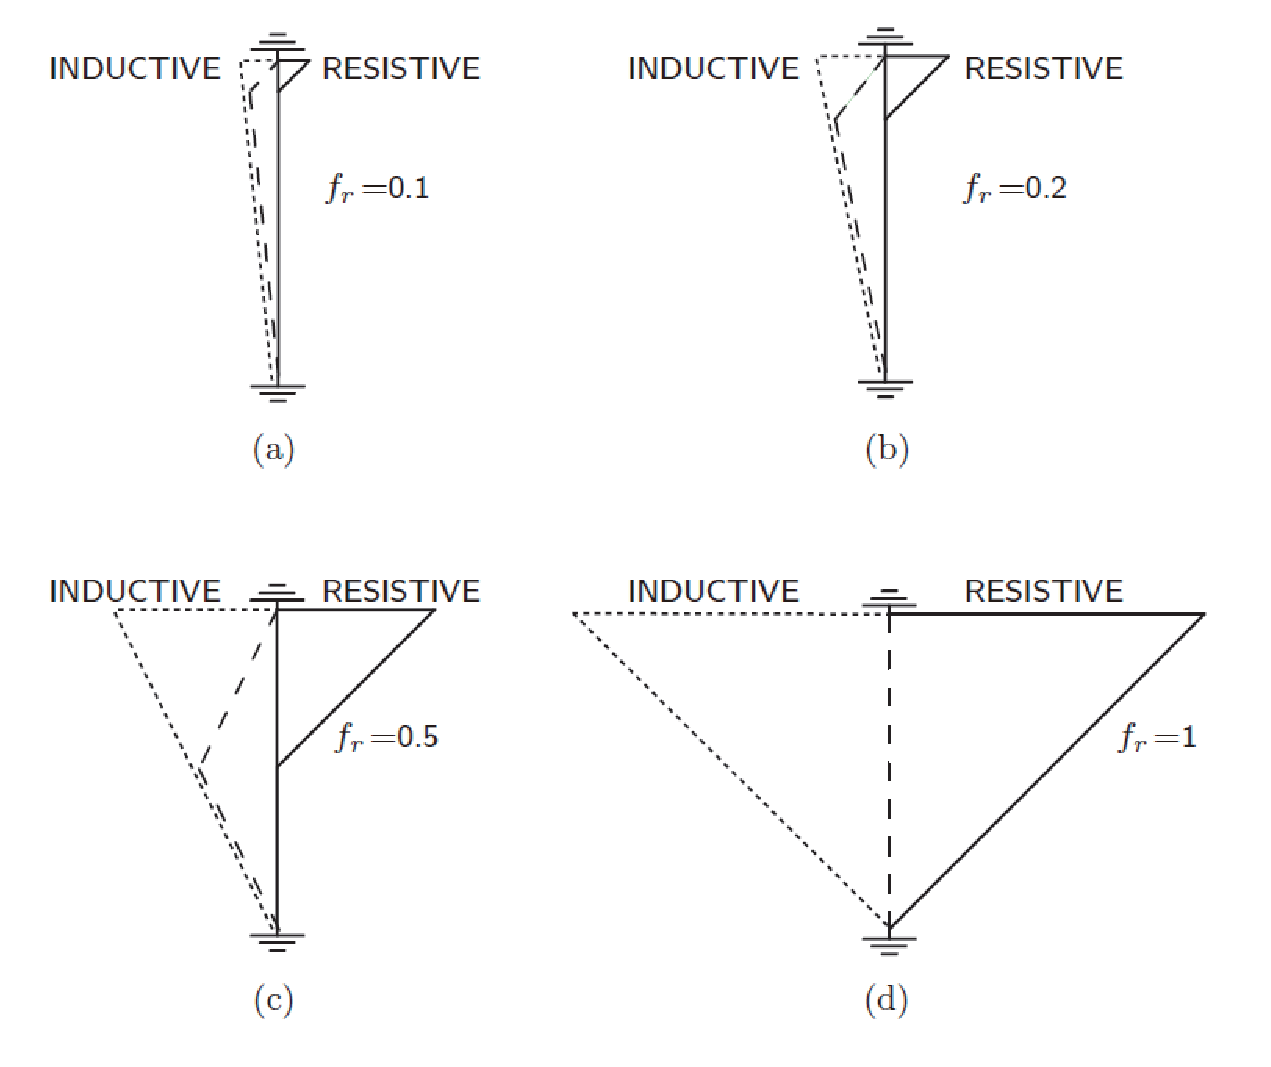
\includegraphics[scale=0.6]{chpt8/figs/fig8.7.eps}
	\caption{Voltage distributions, at constant current, for different normal zone sizes}
\end{figure}



\begin{equation}% 8.38
[V_{in}]_{mx}=f_r(1-f_r)R_{nz}I_{op}
\end{equation}
\begin{equation}% 8.39
[V_{in}]_{mx}=f_r(1-f_r)\frac{\pi(\alpha+1)\rho_m(T_f)a_1}{4A_m}NI_{op}
\end{equation}
\begin{equation}% 8.40a
J_{m_o}^{V}=\frac{2}{f_r(1-f_r)}\left[\frac{F(\alpha,\beta)}{\pi(\alpha^2-1)\beta}\right]\left[\frac{\mu_oV_{bk}I_{op}}{a_{1}^{2}\rho_m(T_f)B_o}\right]
\end{equation}
\begin{equation}% 8.40b
J_{m_o}^{V}=\frac{2}{f_r(1-f_r)}\left[\frac{\sqrt{\ \mathcal{L}(\alpha,\beta)}}{\pi(\alpha+1)}\right]\left[\frac{V_{bk}I_{op}}{\rho_m(T_f)}\sqrt{\frac{2\mu_o}{a_1E_m}}\right]
\end{equation}

\section{正常区传播(NZP)}

\subsection{轴向NZP速度}

\begin{equation}% 8.41a
C_n(T)\frac{\partial T_n}{\partial t}=\frac{\partial}{\partial x}\left[k_n(T)\frac{\partial T_n}{\partial x}\right]+\rho_n(T)J^2
\end{equation}



\begin{figure}
	\centering
	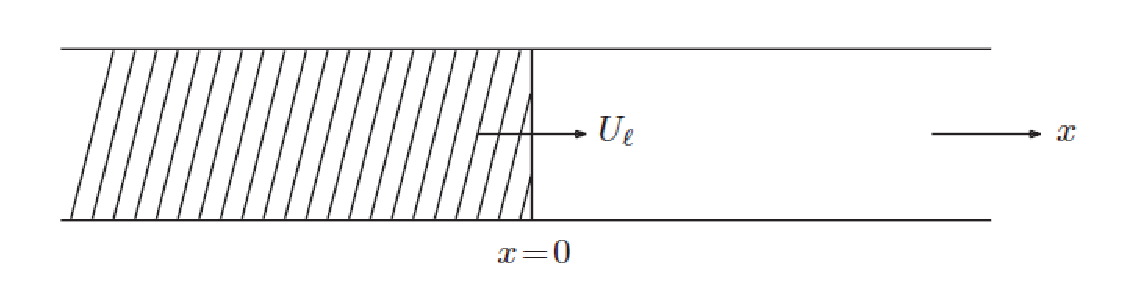
\includegraphics[scale=0.6]{chpt8/figs/fig8.8.eps}
	\caption{One-dimensional normal-to-superconducting boundary}
\end{figure}








\begin{equation}% 8.41b
C_s(T)\frac{\partial T_s}{\partial t}=\frac{\partial}{\partial x}\left[k_s(T)\frac{\partial T_s}{\partial x}\right]
\end{equation}
\begin{equation}% 8.42
\frac{\partial T_n}{\partial t}=\frac{\partial T}{\partial z}\frac{\partial z}{\partial t}=-U_\ell\frac{dT}{dz}
\end{equation}
\begin{equation}% 8.43a
-C_n(T)U_\ell\frac{dT_n}{dz}=\frac{d}{dz}\left[k_n(T)\frac{dT_n}{dz}\right]+\rho_n(T)J^2
\end{equation}
\begin{equation}% 8.43b
-C_s(T)U_\ell\frac{dT_s}{dz}=\frac{d}{dz}\left[k_s(T)\frac{dT_s}{dz}\right]
\end{equation}
\begin{equation}% 8.44a
(z<0)      \frac{d}{dz}\left[k_n(T)\frac{dT_n}{dz}\right]+C_n(T)U_\ell\frac{dT_n}{dz}+\rho_n(T)J^2=0
\end{equation}
\begin{equation}% 8.44b
(z>0)      \frac{d}{dz}\left[k_s(T)\frac{dT_s}{dz}\right]+C_s(T)U_\ell\frac{dT_s}{dz}=0
\end{equation}
\begin{equation}% 8.45a
(z<0)      C_nU_\ell\frac{dT_n}{dz}+\rho_nJ^2=0
\end{equation}
\begin{equation}% 8.45b
(z>0)     k_s\frac{d^2T_s}{dz^2}+C_sU_\ell\frac{dT_s}{dz}=0
\end{equation}
\begin{equation}% 8.46a
T_s(z)=Ae^{-cz}+T_{op}
\end{equation}
\begin{equation}% 8.46b
T_s(z)=(T_t-T_{op})\exp\left(-\frac{C_sU_\ell}{k_s}z\right)+T_{op}
\end{equation}
\begin{equation}% 8.47a
k_n\frac{dT_n}{dz}\mid_0=k_s\frac{dT_s}{dz}\mid_0
\end{equation}
\begin{equation}% 8.47b
-\frac{k_n\rho_nJ^2}{C_nU_\ell}=-C_sU_\ell(T_t-T_{op})
\end{equation}
\begin{equation}% 8.48
U_\ell=J\sqrt{\frac{\rho_nk_n}{C_nC_s(T_t-T_{op})}}
\end{equation}
\begin{equation}% 8.49
U_\ell=J\sqrt{\frac{\rho_n(T_t)k_n(T_t)}{\left[C_n(T_t)-\frac{1}{k_n(T_t)}\frac{dk_n}{dT}\mid_{T_t}\int_{T_{op}}^{T_t}C_s(T)dT\right]\int_{T_{op}}^{T_t}C_s(T)dT}}
\end{equation}
\begin{equation}% 8.50a
U_\ell=\frac{J}{C_o}\sqrt{\frac{\rho_nk_n}{(T_t-T_{op})}}
\end{equation}
\begin{equation}% 8.50b
U_\ell=\frac{J}{C_o(\tilde{T})}\sqrt{\frac{\rho_n(\tilde{T})k_n(\tilde{T})}{(T_t-T_{op})}}
\end{equation}
\begin{equation}% 8.51a
U_\ell=\frac{J_m}{C_{cd}}(\tilde{T})\sqrt{\frac{\rho_m(\tilde{T})k_m(\tilde{T})}{T_t-T_{op}}}
\end{equation}
\begin{equation}% 8.51b
U_\ell\simeq\frac{J_m}{C_m}(\tilde{T})\sqrt{\frac{\rho_m(\tilde{T})k_m(\tilde{T})}{T_t-T_{op}}}
\end{equation}


\begin{figure}
	\centering
	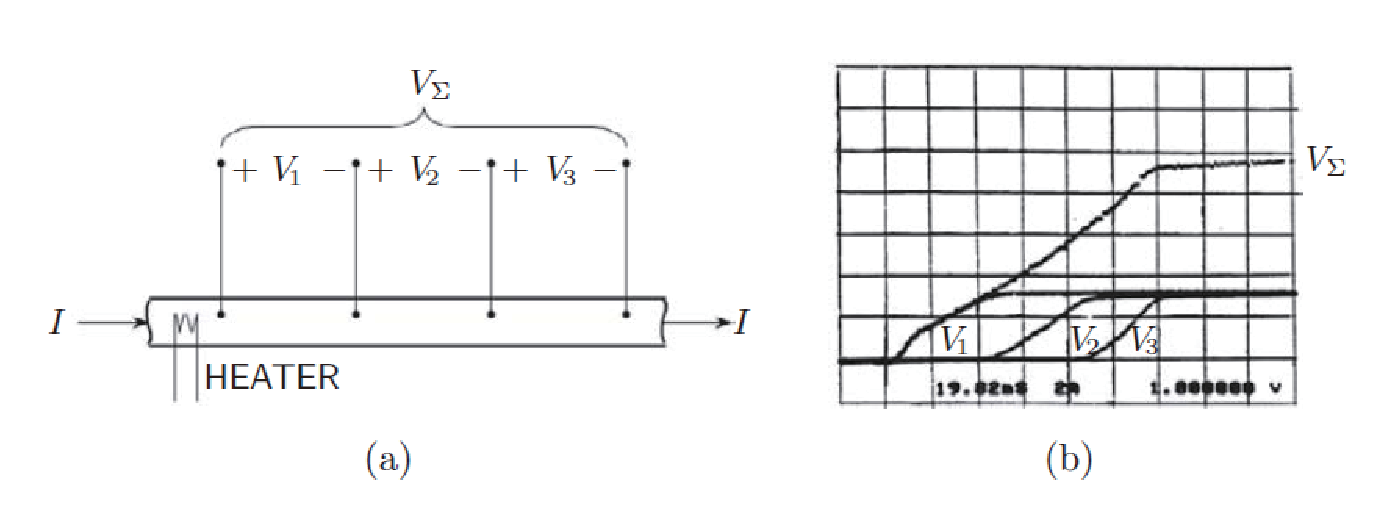
\includegraphics[scale=0.6]{chpt8/figs/fig8.9.eps}
	\caption{(a) Schematic drawing of a setup to experimental}
\end{figure}


\begin{figure}
	\centering
	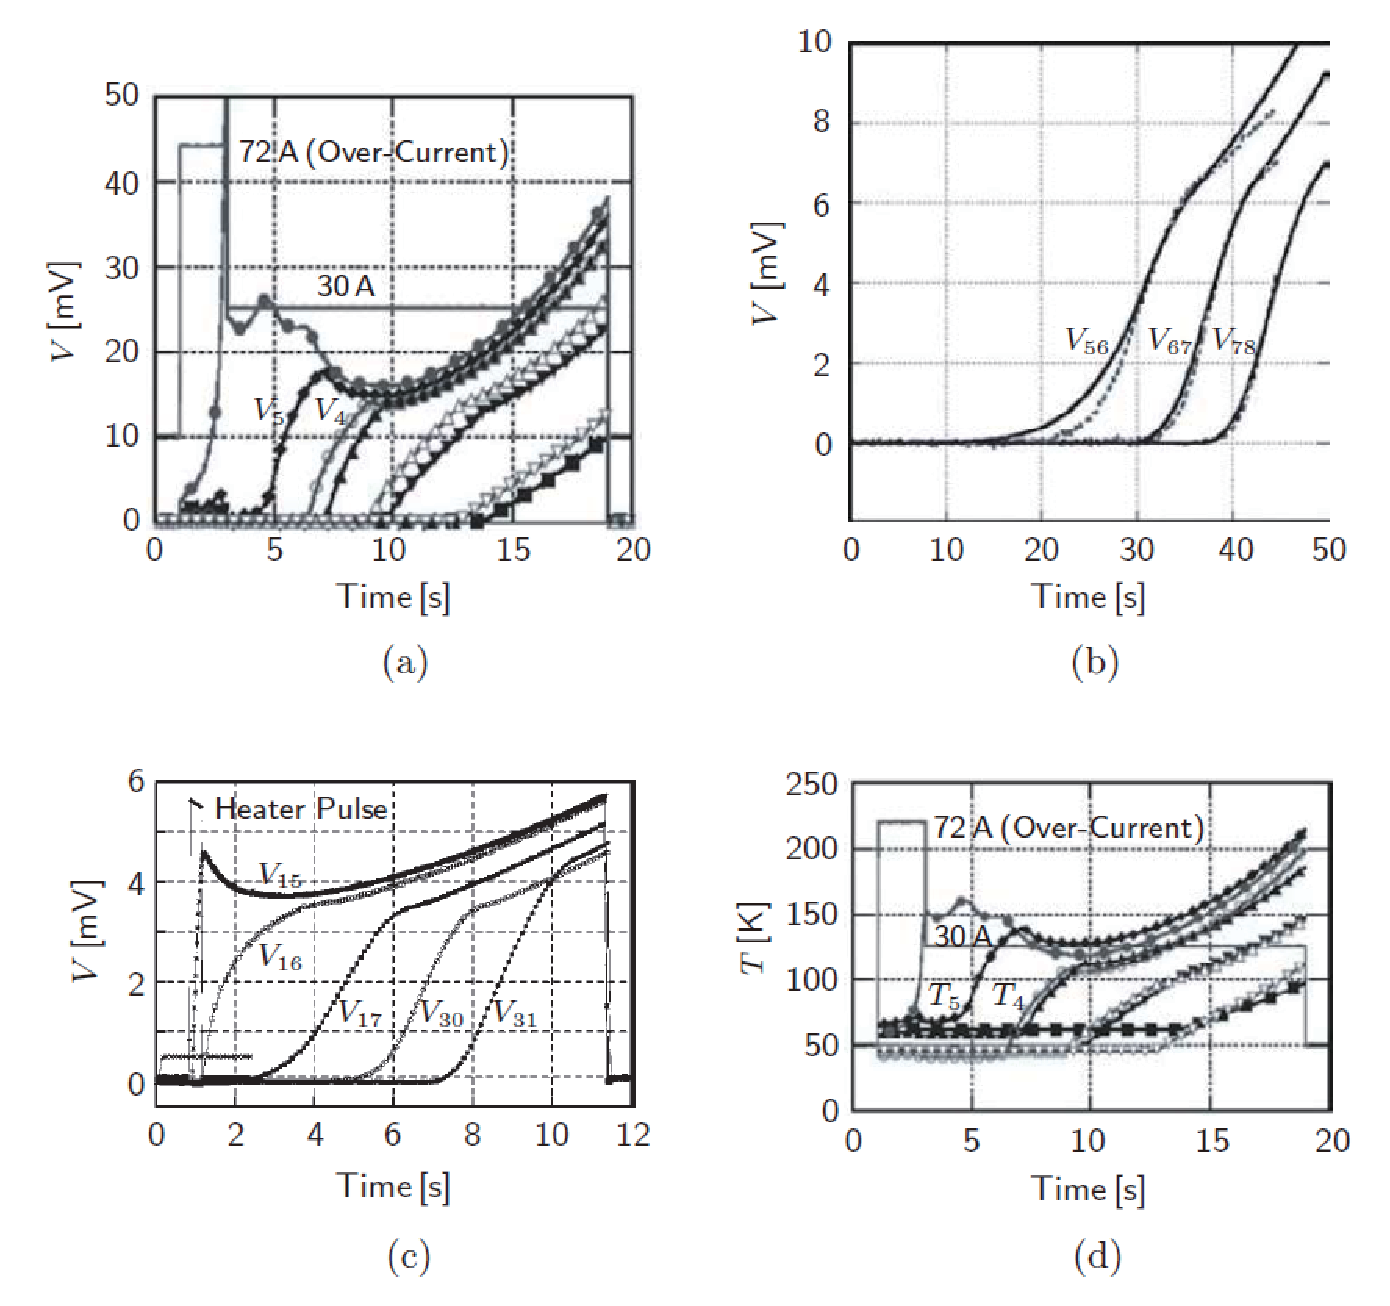
\includegraphics[scale=0.6]{chpt8/figs/fig8.10.eps}
	\caption{Longitudinal NZP signals from YBCO test sample}
\end{figure}


\subsection{“制冷”条件下的NZP}


\subsection{横向匝间速度}



\begin{equation}% 8.52
U_t=U_\ell\sqrt{\frac{1}{2}\left(\frac{\delta_{cd}}{\delta_i}\right)\left[\frac{k_i(\tilde{T})}{k_m(\tilde{T})}\right]}
\end{equation}


\begin{equation}% 8.53
\frac{1}{k_{i}^{\prime}}=\frac{1}{k_i}+R_{th_{ct}^{1}}+R_{th_{ct}^{2}}
\end{equation}



\begin{equation}% 8.54
U_t=U_\ell\sqrt{\frac{1}{2}\left(\frac{\delta_{cd}}{\delta_i}\right)\frac{k_i}{k_m[1+k_i(R_{th_{ct}^{1}}+R_{th_{ct}^{1}})]}}
\end{equation}



\begin{equation}% 8.55
U_t=U_\ell\sqrt{\frac{1}{2}\left(\frac{\delta_{cd}}{\delta_i}\right)\frac{1}{k_m(R_{th_{ct}^{1}}+R_{th_{ct}^{1}})}}
\end{equation}

\begin{figure}
	\centering
	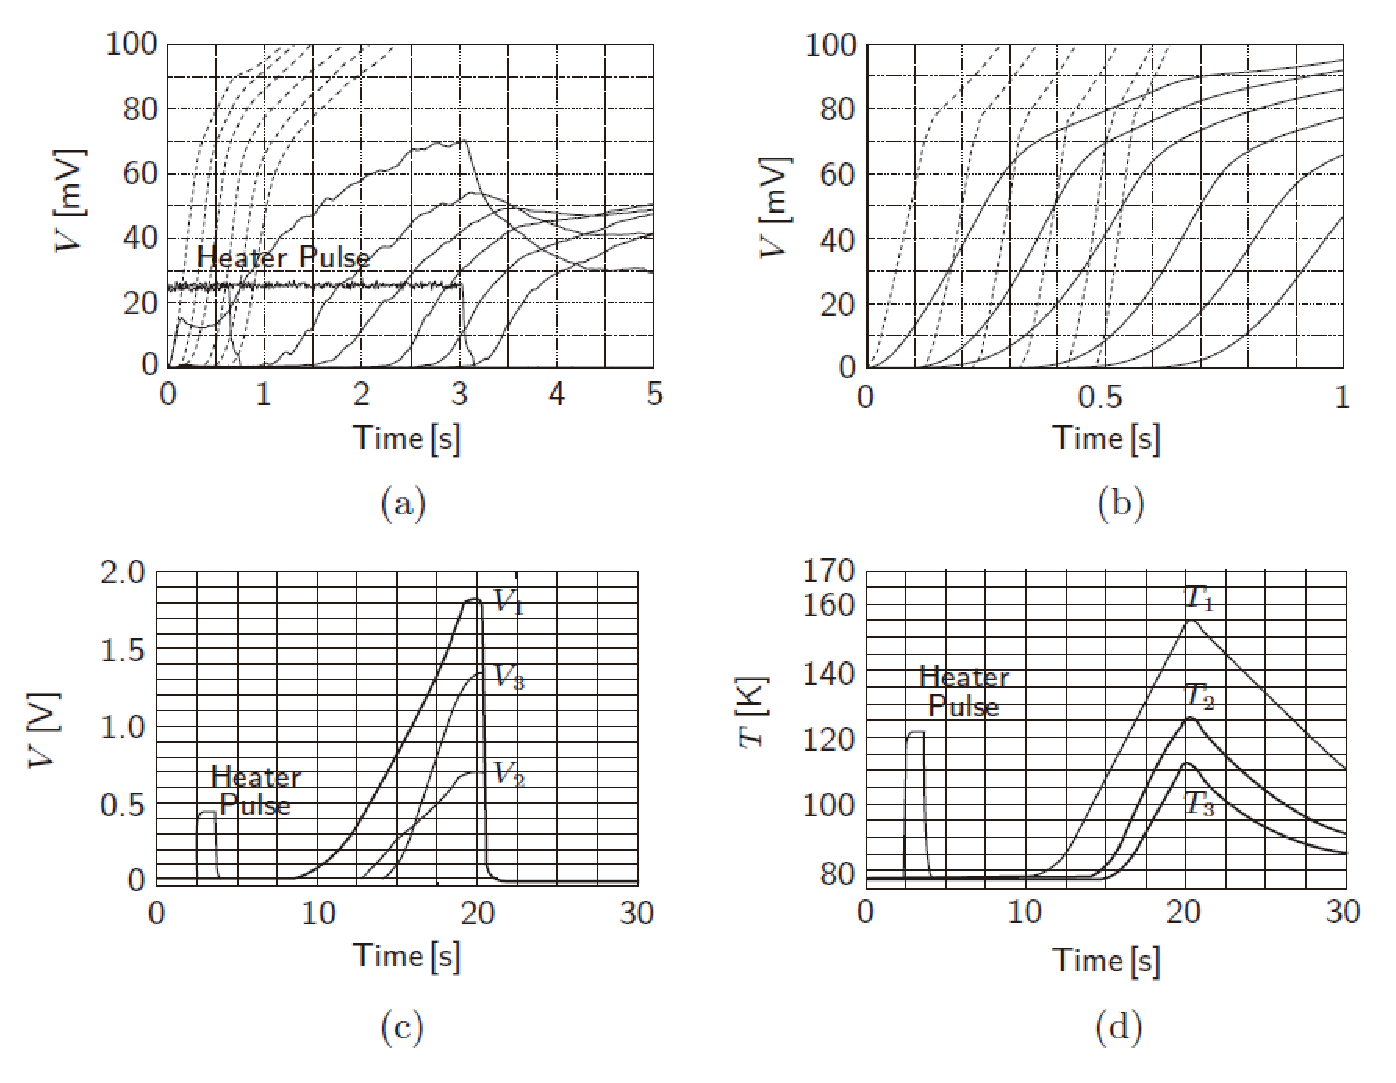
\includegraphics[scale=0.6]{chpt8/figs/fig8.11.eps}
	\caption{Transverse NZP signals from YBCO test asse}
\end{figure}



\subsection{热-流体失超恢复(THQB)}

\subsection{交流损耗诱导的NZP}

\section{计算机仿真}
\begin{equation}% 8.56
\frac{d_{cd}}{U_t}\ll\frac{2\pi a_1}{U_\ell}
\end{equation}


\begin{figure}
	\centering
	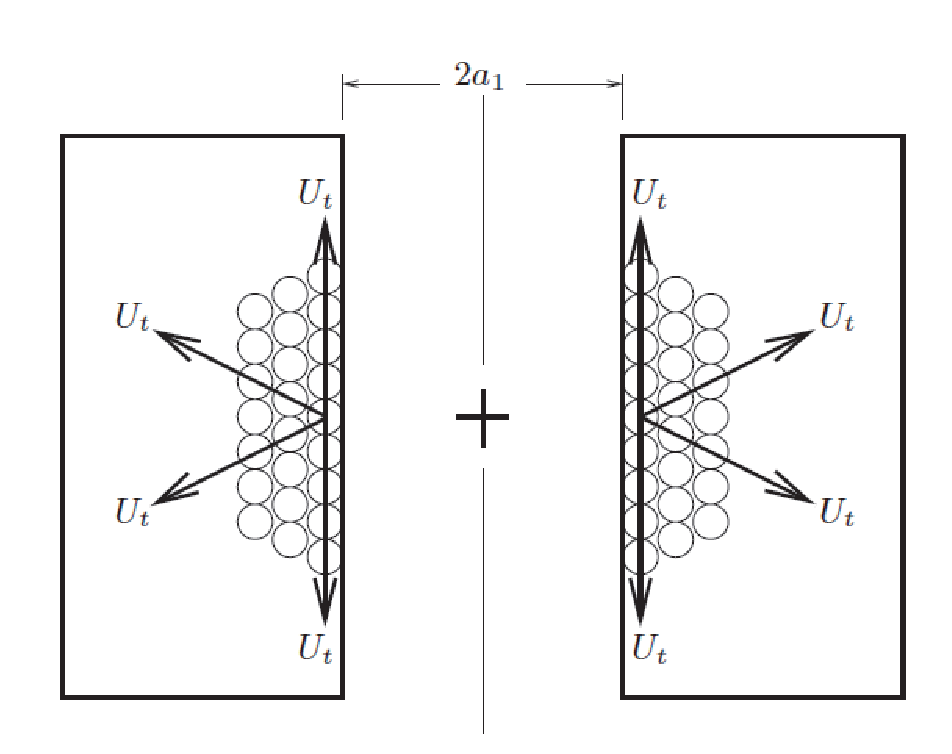
\includegraphics[scale=0.6]{chpt8/figs/fig8.12.eps}
	\caption{Quenching in an adiabatic, solenoidal winding}
\end{figure}

\section{自保护磁体}

\subsection{尺度限制}

\begin{equation}% 8.57
\frac{a_1(\alpha-1)}{U_t}<\tau_{dg}
\end{equation}
\begin{equation}% 8.58
\frac{a_1(\alpha-1)}{U_t}=\frac{Z(T_f,T_i)}{J_{m_o}^{2}}
\end{equation}
\begin{equation}% 8.59
[a_1(\alpha-1)]_{ah}^{i}=\frac{Z(T_f,T_i)}{J_{m_o}C_m(\tilde{T})}\sqrt{\frac{\rho_m(\tilde{T})k_i(\tilde{T})\delta_{cd}}{2\delta_i(T_t-T_{op})}}
\end{equation}


\begin{subequations}% 8.60a 8.60b 8.60c
	\begin{align*}
[a_1(\alpha-1)]_{ah}^{sh}=U_t\left(\frac{L}{R_{nz}}\right) \\
&=\frac{J_{m_o}}{C_n(\tilde{T})}\sqrt{\frac{\rho_m(\tilde{T})k_i(\tilde{T})\delta_{cd}}{2\delta_i(T_t-T_{op})}}\left(\frac{L}{R_{nz}}\right)  \\
&=\frac{J_{m_o}}{C_n(\tilde{T})}\sqrt{\frac{\rho_m(\tilde{T})k_i(\tilde{T})\delta_{cd}}{2\delta_i(T_t-T_{op})}}\times 
\frac{4A_m}{f_r\pi(\alpha+1)\rho_m(T_f)}\sqrt{\frac{\mu_o\mathcal{L}(\alpha,\beta)L}{a_1}}\\
[a_1(\alpha-1)]_{ah}^{sh}&=\frac{1}{C_m(\tilde{T})}\sqrt{\frac{\rho_m(\tilde{T})k_i(\tilde{T})\delta_{cd}}{2\delta_i(T_t-T_{op})}}\times 
\frac{4}{f_r\pi(\alpha+1)\rho_m(T_f)}\sqrt{\frac{2\mu_o\mathcal{L}(\alpha,\beta)E_m}{a_1}}
\end{align*}
\end{subequations}



\section{孤立磁体的被动保护}

\begin{equation}% 8.61
\frac{E_r}{E_m}=\frac{0.5\zeta(1-k)+(1+k)}{\zeta+(1+k)}
\end{equation}


\begin{figure}
	\centering
	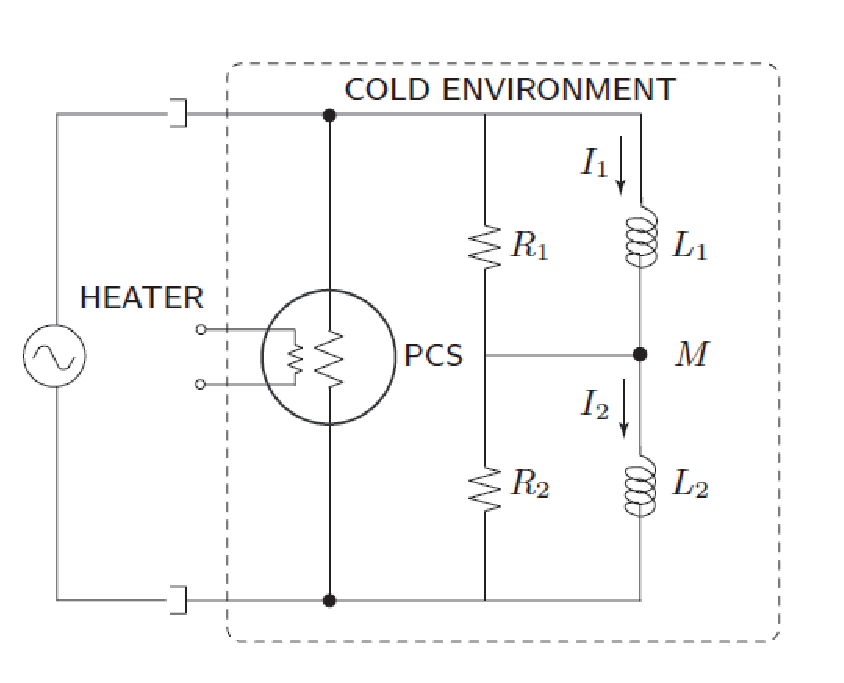
\includegraphics[scale=0.6]{chpt8/figs/fig8.13.eps}
	\caption{Circuit for an “isolated,” persistent-mode 2-coil magnet.}
\end{figure}





\begin{equation}% 8.62a
\frac{I_1(t)}{I_0}=\frac{R(1+k)^2}{2r}\exp\left(-\frac{Rt}{2L}\right)\left[1-\frac{R(1+k)^2}{2r}\right]\exp\left[-\frac{rt}{(1-k^2)L}\right]
\end{equation}
\begin{equation}% 8.62b
\frac{I_2(t)}{I_0}=(1+k)\exp\left(-\frac{Rt}{2L}\right)-k\exp\left[-\frac{rt}{(1-k^2)L}\right]
\end{equation}


\begin{figure}
	\centering
	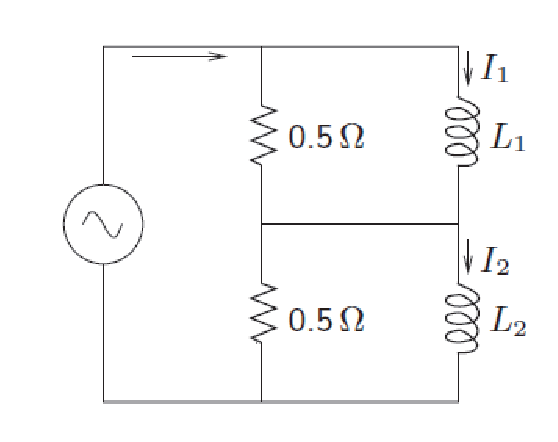
\includegraphics[scale=0.6]{chpt8/figs/fig8.14.eps}
	\caption{2-Coil Magnet circuit}
\end{figure}





\begin{figure}
	\centering
	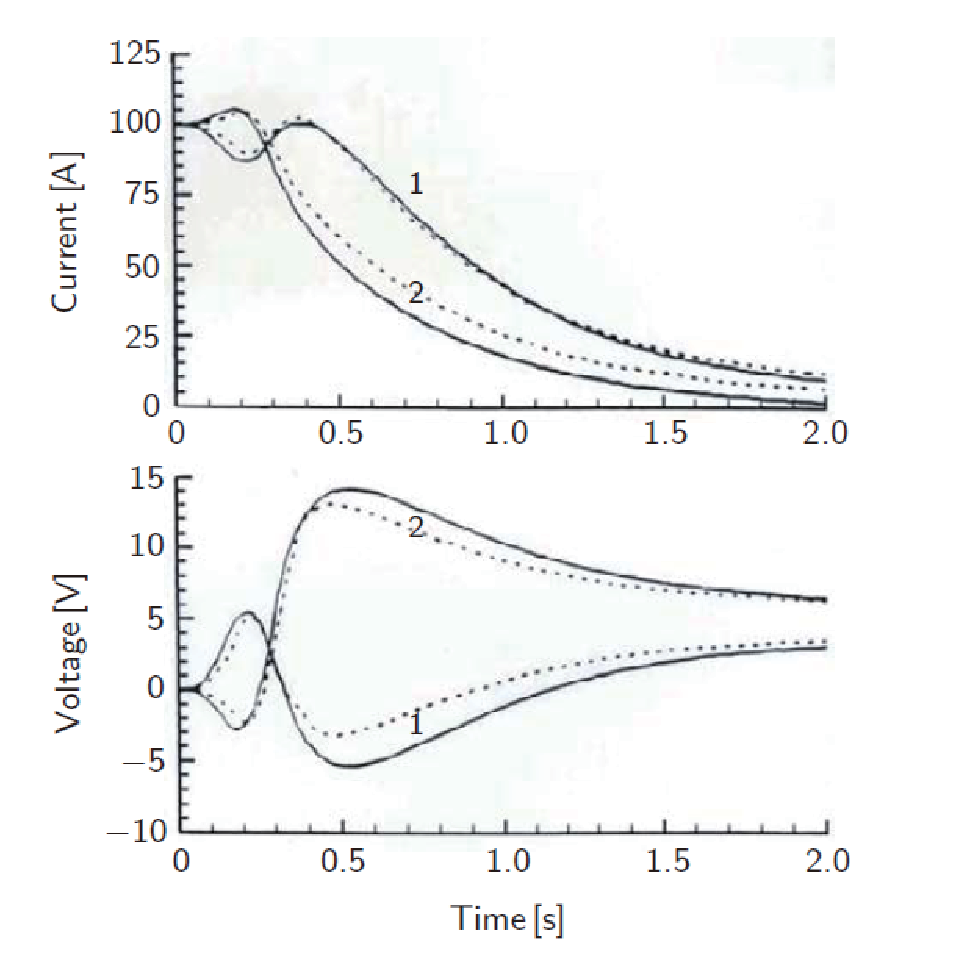
\includegraphics[scale=0.6]{chpt8/figs/fig8.15.eps}
	\caption{Current and voltage vs. time traces of Coil 1 }
\end{figure}







\begin{equation}% 8.63
E_d=E_m+E_s-E_{R1}-E_{R2}
\end{equation}

\begin{align*}% page500第一个
E_s&=(100\ \mathrm{A})\int_{0}^{0.4\ \mathrm{s}}[V_1(t)+V_2(t)]dt+(10\ \mathrm{V})\int_{0.4\ \mathrm{s}}^{2\ \mathrm{s}}\left[I_1(t)+\frac{V_1(t)}{R_1}\right]dt \\
&\simeq 200\ \mathrm{J}+650\ \mathrm{J}\simeq 850\ \mathrm{J}
\end{align*}


\begin{equation}% page500 第二个和第三个
E_{R1}=\frac{1}{R_1}\int_{0}^{2\ \mathrm{s}}V_1(t)^2dt\simeq 50\ \mathrm{J} 
E_{R2}=\frac{1}{R_2}\int_{0}^{2\ \mathrm{s}}V_2(t)^2dt\simeq 300\ \mathrm{J}
\end{equation}

\begin{equation}% page500第四个
\mathcal{V}_{cd}[h_{cu}(T_f)-h_{cu}(T_{op})]\simeq(694\ \mathrm{cm^3})[h_{cu}(T_f)]=5500\ \mathrm{J}
\end{equation}




\begin{figure}
	\centering
	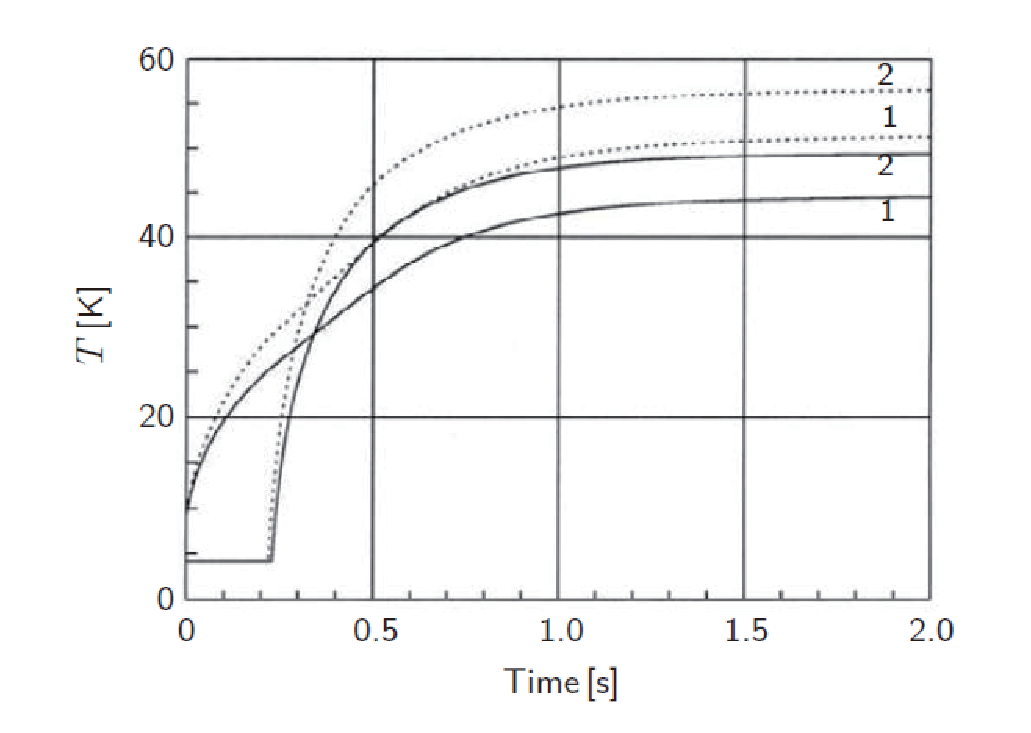
\includegraphics[scale=0.6]{chpt8/figs/fig8.16.eps}
	\caption{Spatially averaged temperature vs. time plots for Coils 1 and 2 }
\end{figure}







\section{主动保护}
\subsection{过热}
\begin{equation}% page501 8.7
e_{mr}\equiv\frac{E_m}{V_r}=\frac{2(\alpha-1)\beta\mathcal{L}(\alpha,\beta)}{f_r\pi(\alpha+1)F^2(\alpha,\beta)}\left(\frac{B_{o}^{2}}{2\mu_o}\right)
\end{equation}


\subsection{多线圈磁体中的过压}


\subsection{主动保护技术:检测-抑制}

\begin{equation}% page502 8.18b
Z(T_f,T_i)=\frac{J_{m_o}E_m}{A_{cd}V_D}
\end{equation}

\begin{figure}
	\centering
	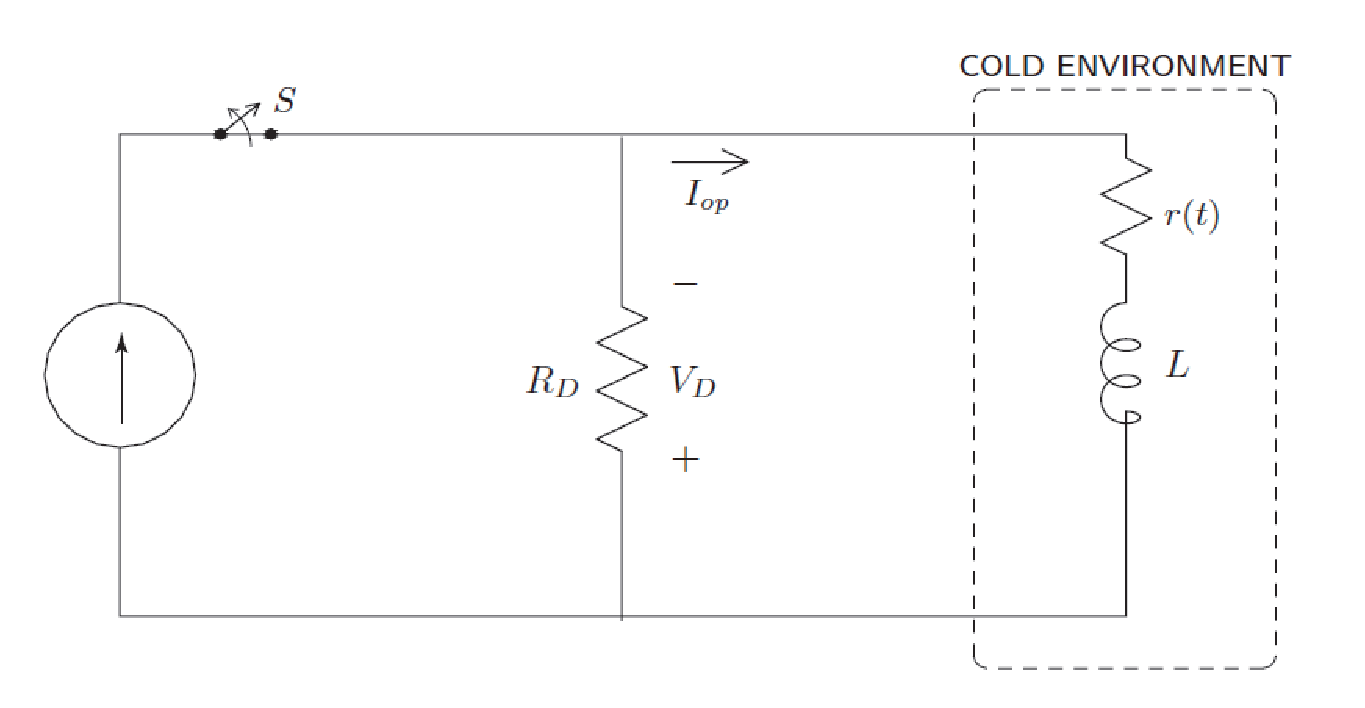
\includegraphics[scale=0.6]{chpt8/figs/fig8.17.eps}
	\caption{Magnet circuit for detect-and-dump active protection}
\end{figure}



\begin{equation}% page503 8.19
J_{m_o}^{D}=\frac{A_{cd}Z(T_f,T_i)V_D}{E_m}
\end{equation}



\begin{equation}% 8.65
V_D=\frac{J_{m_o}E_m}{A_{cd}Z(T_f,T_i)}
\end{equation}
\begin{equation}% 8.66a 8.66b
Z(T_f,T_i)=\left(\frac{A_m}{A_{cd}}\right)(J_{m_o}^{2}\tau_{dl}+\frac{1}{2}J_{m_o}^{2}\tau_{dg})
=\left(\frac{A_m}{A_{cd}}\right)(\tau_{dl}+\frac{1}{2}\tau_{dg})J_{m_o}^{2}
\end{equation}






\subsection{主动保护技术:检测-激活加热器}

\begin{figure}
	\centering
	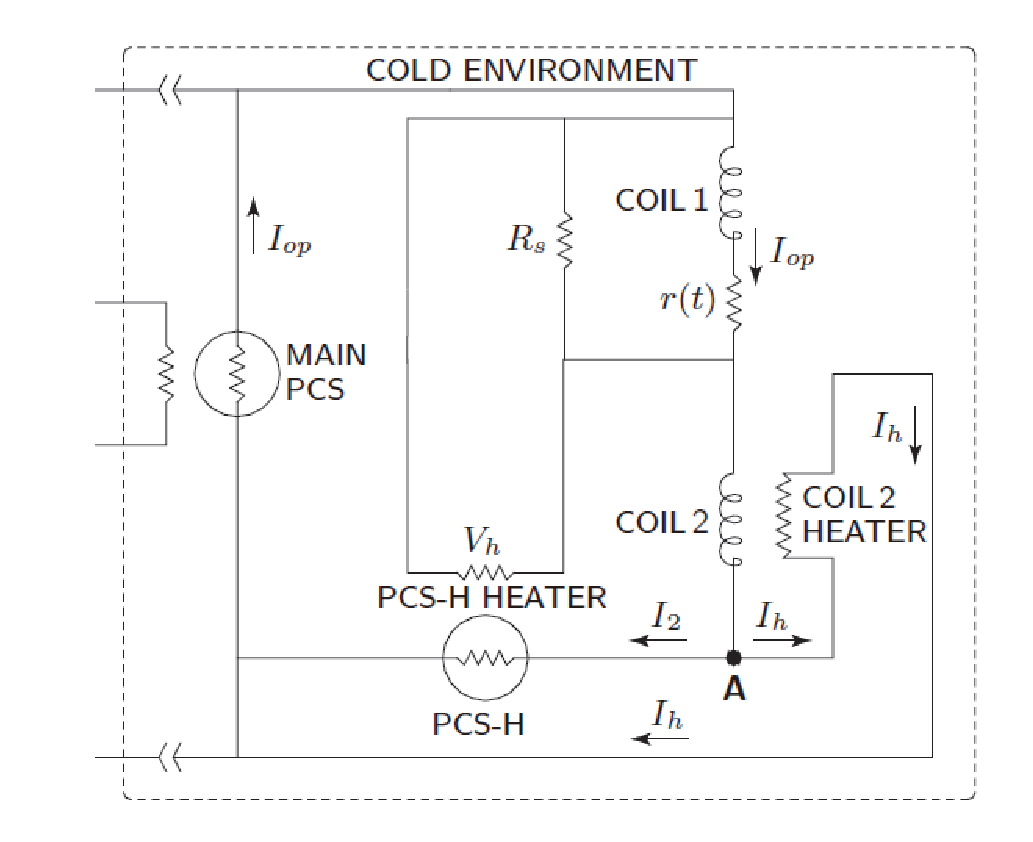
\includegraphics[scale=0.6]{chpt8/figs/fig8.18.eps}
	\caption{Magnet circuit with passive activate-the-heater protection.}
\end{figure}




\subsection{失超电压保护技术:基本电桥}


\begin{figure}
	\centering
	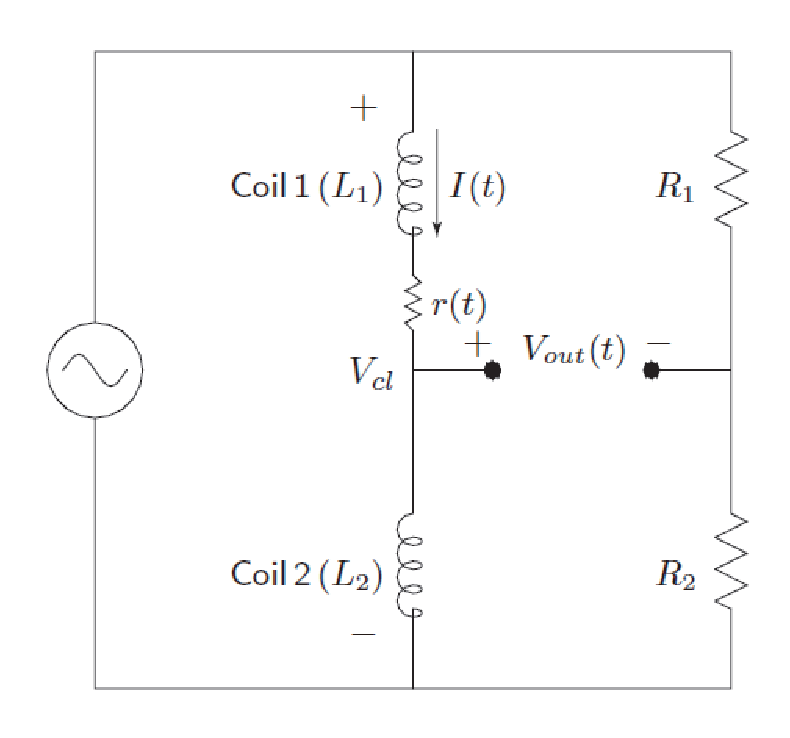
\includegraphics[scale=0.6]{chpt8/figs/fig8.19.eps}
	\caption{Bridge circuit voltage detection technique}
\end{figure}


\begin{equation}% 8.67a
V_{cl}(t)=L_1\frac{dI(t)}{dt}+rI(t)+L_2\frac{dI(t)}{dt}
\end{equation}
\begin{equation}% 8.67b
i_R(t)=\frac{V_{cl}(t)}{R_1+R_2}
\end{equation}
\begin{equation}% 8.67c
V_{out}(t)=L_1\frac{dI(t)}{dt}+rI(t)-R_1i_R(t)
\end{equation}


\begin{align}% 8.68
V_{out}(t)&=L_1\frac{dI(t)}{dt}+rI(t) 
-\frac{R_1}{R_1+R_2}\left[L_1\frac{dI(t)}{dt}+rI(t)+L_2\frac{dI(t)}{dt}\right] \\\notag
&=\left(\frac{R_2}{R_1+R_2}\right)L_1\frac{dI(t)}{dt} 
-\left(\frac{R_1}{R_1+R_2}\right)L_2\frac{dI(t)}{dt}+\left(\frac{R_2}{R_1+R_2}\right)rI(t)
\end{align}



\begin{equation}% 8.69
\left(\frac{R_2}{R_1+R_2}\right)L_1\frac{dI(t)}{dt}-\left(\frac{R_1}{R_1+R_2}\right)L_2\frac{dI(t)}{dt}=0
\end{equation}


\begin{equation}% 8.70
V_{out}(t)=\left(\frac{R_2}{R_1+R_2}\right)rI(t)
\end{equation}


\section{专题}

\subsection{问题8.1:大型超导磁体的回温}
\begin{equation}% 8.71a 8.71b
\mathcal{V}C_{cd}(T)\frac{dT}{dt}=\frac{\rho_m(T)\ell_{cd}}{A_m}I_{o}^{2} 
=\frac{A_m}{\rho_m(T)\ell_{cd}}V_{o}^{2}
\end{equation}

\subsubsection{问题8.1之解}
\begin{align*}% page508 S1.1
\Delta t_{\omega}^{I}\mid_{10\ \mathrm{K}}^{300\ \mathrm{K}}&=\frac{\mathcal{V}_{cd}A_m}{\ell_{cd}I_{o}^{2}}\int_{10\ \mathrm{K}}^{300\ \mathrm{K}}\frac{C_{cu}(T)}{\rho_m{cu}(T)}dT \\
&=\frac{\mathcal{V}_{cd}A_m}{\ell_{cd}I_{o}^{2}}Z(T_f=300\ \mathrm{K},T_i=10\ \mathrm{K})
\end{align*}


\begin{align*}% page508 S1.2
\Delta t_{\omega}^{I}\mid_{10\mathrm{K}}^{300\mathrm{K}}&=\frac{(0.4\ \mathrm{m^3})(1.5\times 10^{-5}\ \mathrm{m^2})(15.1\times 10^{16}\ \mathrm{A^2s/m^4})}{(1\times 10^4\ \mathrm{m})(25\ \mathrm{A})^2} \\
&\simeq 1.45\times 10^5\ \mathrm{s}\simeq 40\ \mathrm{h}\simeq 1\frac{2}{3}\ \mathrm{days} 
\end{align*}


\begin{align*}% page508 S1.3
\Delta t_{\omega}^{I}\mid_{10\mathrm{K}}^{300\mathrm{K}}&=\frac{\mathcal{V}_{cd}\ell_{cd}}{A_mV_{o}^{2}}\int_{10\ \mathrm{K}}^{300\ \mathrm{K}}C_{cu}(T)\rho_m{cu}(T)dT \\
&=\frac{\mathcal{V}_{cd}\ell_{cd}}{A_mV_{o}^{2}}Y(T_f=300\ \mathrm{K},T_i=10\ \mathrm{K})
\end{align*}


\begin{align*}% page508 S1.4
\Delta t_{\omega}^{I}\mid_{10\mathrm{K}}^{300\mathrm{K}}&=\frac{(0.4\ \mathrm{m^3})(1\times 10^4\ \mathrm{m})(7.25\ \mathrm{V^2s/m^2})}{(1.5\times 10^{-5}\ \mathrm{m^2})(25\ \mathrm{V})^2} \\
&=3.1\times 10^6\ \mathrm{s}\simeq 860\ \mathrm{h}\simeq 36\ \mathrm{days} 
\end{align*}


\begin{align*}% page509 S1.5
\Delta t_{\omega}^{I}\mid_{10\mathrm{K}}^{50\mathrm{K}}&=\frac{(0.4\ \mathrm{m^3})(1.5\times 10^{-5}\ \mathrm{m^2})(4.5\times 10^{16}\ \mathrm{A^2s/m^4})}{(1\times 10^4\ \mathrm{m})(100\ \mathrm{A})^2} \\
&\simeq 2.7\times 10^3\ \mathrm{s}=45\ \mathrm{min}
\end{align*}


\begin{equation}% page509 S1.6
\Delta t_{\omega}^{I}\mid_{50\mathrm{K}}^{300\mathrm{K}}=\frac{(0.4\ \mathrm{m^3})(1\times 10^4\ \mathrm{m})(7.25\ \mathrm{J\Omega/m^2})}{(1.5\times 10^{-5}\ \mathrm{m^2})(100\ \mathrm{V})^2} 
=1.93\times 10^5\ \mathrm{s}=54\ \mathring{h}
\end{equation}
\begin{equation}% page509 S1.7
\Delta t_{\omega}^{I}\mid_{80\mathrm{K}}^{300\mathrm{K}}\simeq 0.7\times 10^5\ \mathrm{s}\sim 20\ \mathrm{h}
\end{equation}
\begin{equation}% page509 S1.8
\Delta t_{\omega}^{I}\mid_{80\mathrm{K}}^{300\mathrm{K}}\simeq 3\times 10^6\ \mathrm{s}\simeq 830\ \mathrm{h}\simeq 35\ \mathrm{days}
\end{equation}



\subsection{问题8.2:6 kA气冷HTS引线的保护}


\subsubsection{问题8.2之解}
\begin{equation}% 8.66b
Z(T_f,T_i)=\left(\frac{A_m}{A_{cd}}\right)(\tau_{dl}+\frac{1}{2}\tau_{dg})J_{o}^{2}
\end{equation}
\begin{equation}% page510 S.1
Z(T_f,T_i)=\left(\frac{\gamma_{m/s}}{1+\gamma_{m/s}}\right)(\tau_{dl}+\frac{1}{2}\tau_{dg})J_{o}^{2}
\end{equation}
\begin{equation}% page510 第三个
Z(T_f,T_i)=(12.5\ \mathrm{s})\left(\frac{2}{3}\right)(3.46\times 10^7\ \mathrm{A/m^2})^2\simeq 1\times 10^{16}\ \mathrm{A^2s/m^4}
\end{equation}



\subsection{问题8.3:制冷机制冷的NbTi磁体的保护}

\subsubsection{问题8.3之解}
\begin{equation}% page511 第一个
I_{op}=(6.25\times 10^7\ \mathrm{A/m^2})\frac{(10\times 10^{-3}\ \mathrm{m})(3\times 10^{-3}\ \mathrm{m})4}{(1+4)}=1500\ \mathrm{A}
\end{equation}
\begin{equation}% 8.72
V_D=\frac{J_{m_o}E_m}{A_{cd}Z(T_f,T_i)}
\end{equation}
\begin{equation}% page511 S3.1
V_D=\frac{(6.25\times 10^7\ \mathrm{A/m^2})^2(10\times 10^6\ \mathrm{J})}{(3\times 10^{-5}\ \mathrm{m^2})(6.7\times 10^{16}\ \mathrm{A^2s/m^4})} 
=310\ \mathrm{V}
\end{equation}



\subsection{问题8.4:混合III SCM的“热点”温度}
\begin{equation}% 8.73
r(t)=r_0+\eta t
\end{equation}
\begin{equation}% 8.74
I(t)=I_{op}\exp\left[-\frac{(R_D+r_0)}{L}t-\frac{\eta}{2L}t^2\right]
\end{equation}


\subsubsection{问题8.4之解}

\begin{equation}% page513 8.16c
Z(T_f,T_i)=\left(\frac{\gamma_{m/s}}{1+\gamma_{m/s}}\right)J_{m_o}^{2}\left(\frac{L}{2R_D}\right)
\end{equation}
\begin{equation}% page513 S4.1
J_{m_o}=\frac{I_{op}}{A_m}=\left(\frac{\gamma_{m/s}+1}{\gamma_{m/s}}\right)\frac{I_{op}}{ab}
\end{equation}
\begin{equation}% page513 S4.2
J_{m_o}=\left(\frac{5.1}{4.1}\right)\frac{(2230\ \mathrm{A})}{(9.49\times 10^{-3}\ \mathrm{m})(4.52\times 10^{-3}\ \mathrm{m})} 
=6.47\times 10^7\ \mathrm{A/m^2}
\end{equation}
\begin{equation}% page513 S4.2后第一个
Z(T_f,4\ \mathrm{K})=\left(\frac{5.1}{4.1}\right)(6.47\times 10^7\ \mathrm{A/m^2})^2\left(\frac{8\ \mathrm{H}}{2\times 0.3\Omega}\right)
\end{equation}
\begin{equation}% page513 S4.2后第二个
Z(T_f,4\ \mathrm{K})=4.5\times 10^{16}\ \mathrm{A^2s/m^4}
\end{equation}
\begin{equation}% page513 S4.3
L\frac{dI(t)}{dt}+(R_D+R_0+\eta t)I(t)=0
\end{equation}
\begin{equation}% page513 S4.4
\frac{dI(t)}{dt}=-\frac{(R_D+R_0+\eta t)}{L}dt
\end{equation}
\begin{equation}% page513 S4.5
\ln\left[\frac{I(t)}{I_{op}}\right]=-\frac{(R_D+R_0)}{L}t-\frac{\eta}{2L}t^2
\end{equation}
\begin{equation}% 8.74
I(t)=I_{op}\exp\left[-\frac{(R_D+R_0)}{L}t-\frac{\eta}{2L}t^2\right]
\end{equation}
\begin{equation}% page514 S4.6
E_{sm}\int_{0}^{\infty}r(t)I_{0}^{2}\exp\left[-\frac{2(R_D+R_0)}{L}t-\frac{\eta}{L}t^2\right]dt
\end{equation}

\subsection{讨论8.1:失超电压探测——一个变种}


\begin{figure}
	\centering
	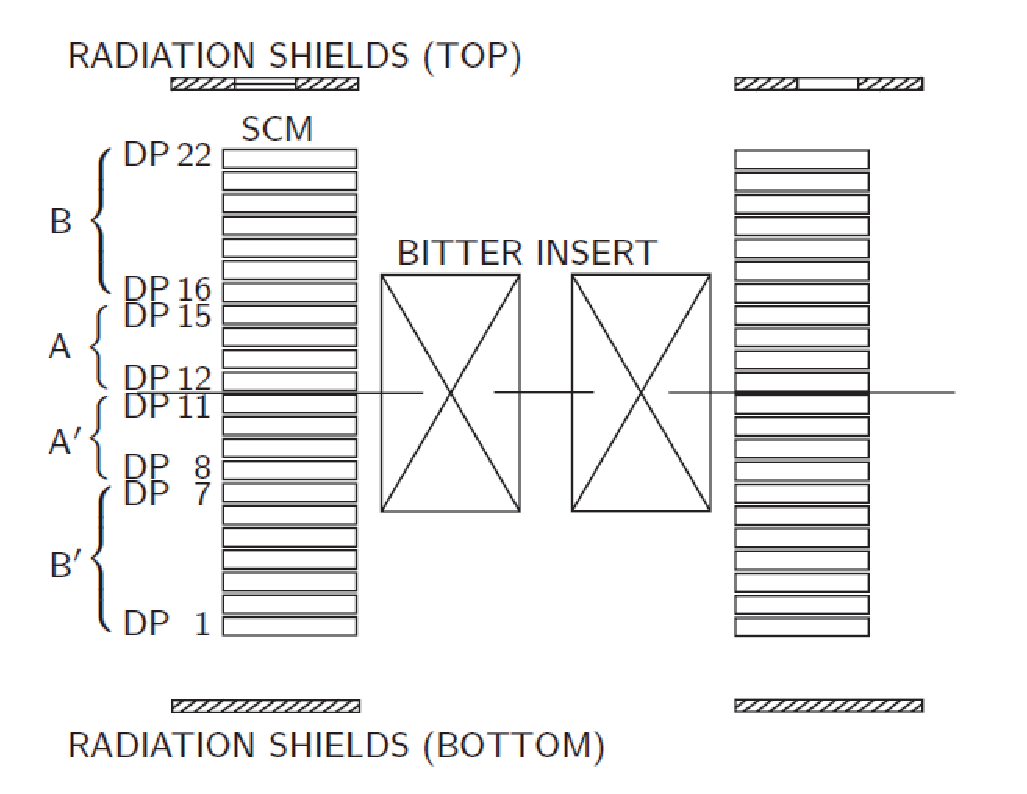
\includegraphics[scale=0.6]{chpt8/figs/fig8.20.eps}
	\caption{Schematic arrangement of Hybrid II with a Bitter insert}
\end{figure}




\begin{equation}% 8.75
V_{out}(t)=\sum_{n=1}^{11}[\alpha_{2n-1}V_{2n-1}(t)-\alpha_{2n}V_{2n}(t)]
\end{equation}

\begin{figure}
	\centering
	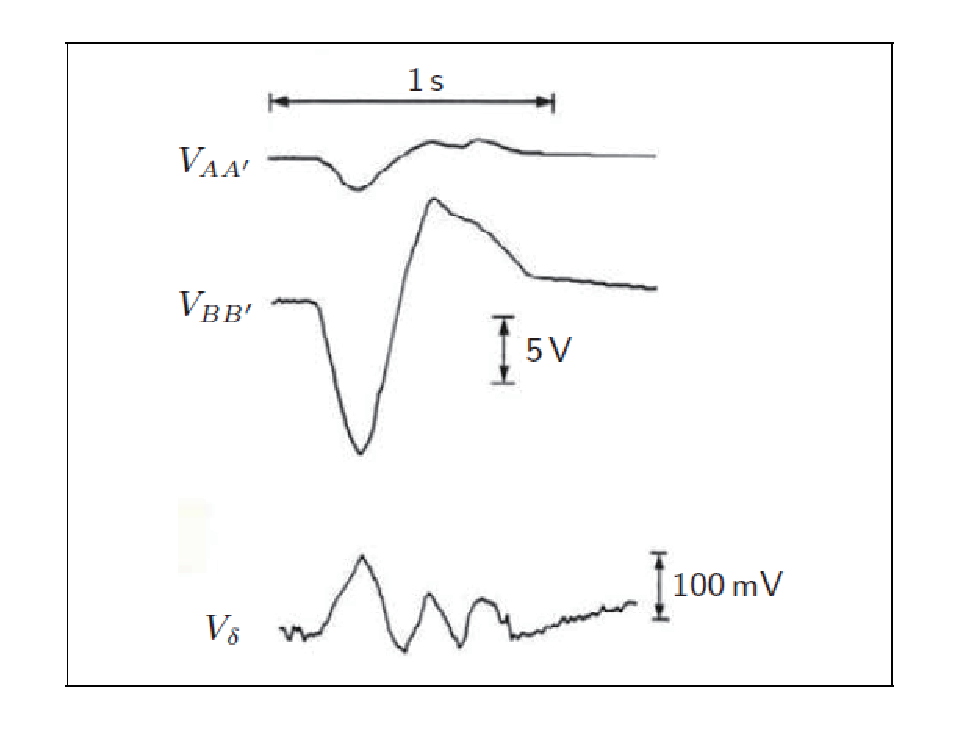
\includegraphics[scale=0.6]{chpt8/figs/fig8.21.eps}
	\caption{Measured unbalanced voltages from an insert trip in Hybrid II}
\end{figure}



\subsection{问题8.5:抑制电阻的设计}
\begin{equation}% 8.76a
\ell=\sqrt{\frac{E_mR_D}{\rho C_p\Delta T}}
\end{equation}
\begin{equation}% 8.76b
\omega\delta=\sqrt{\frac{\rho E_m}{R_DC_p\Delta T}}
\end{equation}

\begin{figure}
	\centering
	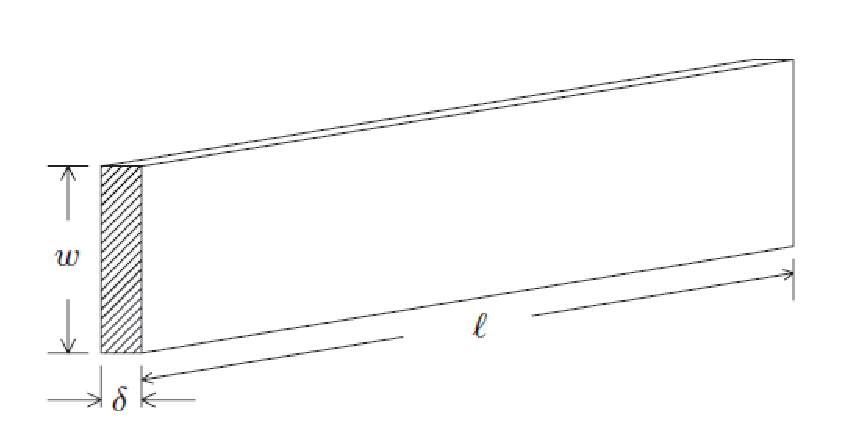
\includegraphics[scale=0.6]{chpt8/figs/fig8.22.eps}
	\caption{Schematic drawing of a dump resistor in the form of a}
\end{figure}






\subsubsection{问题8.5之解}

\begin{equation}% page518 S5.1a
R_D-\frac{\rho\ell}{\omega\delta}
\end{equation}
\begin{equation}% page518 S5.1b
\omega\delta=\frac{\rho\ell}{R_D}
\end{equation}
\begin{equation}% page518 S5.2a
E_m=\ell\omega\delta C_p\Delta T
\end{equation}
\begin{equation}% page518 S5.2b
\omega\delta=\frac{E_m}{\ell C_p\Delta T}
\end{equation}
\begin{equation}% 8.76a
\omega\delta=\sqrt{\frac{\rho E_m}{R_DC_p\Delta T}}
\end{equation}
\begin{equation}% page518 倒数第二个
\ell\simeq\sqrt{\frac{(2\times 10^7\ \mathrm{J})(0.3\Omega)}{(10^{-6}\ \mathrm{\Omega m})(4\times 1066\ \mathrm{J/m^2K})(200\ \mathrm{K})}} 
=86.6\ \mathrm{m}
\end{equation}
\begin{align*}% page518 最后一个
\omega\delta&\simeq\sqrt{\frac{(10^{-6}\ \mathrm{\Omega m})(2\times 10^7\ \mathrm{J})}{(0.3\Omega)(4\times 10^6\ \mathrm{J/m^2K})(200\ \mathrm{K})}} \\
&\simeq 2.9\times 10^{-4}\ \mathrm{m^2}\simeq 290\ \mathrm{mm^2}
\end{align*}


\subsection{讨论8.2:磁体的“缓慢”放电模式}
\begin{equation}% 8.77a
\frac{dI_m(t)}{dt}=-\frac{I_m(t)}{\tau_m}
\end{equation}


\begin{figure}
	\centering
	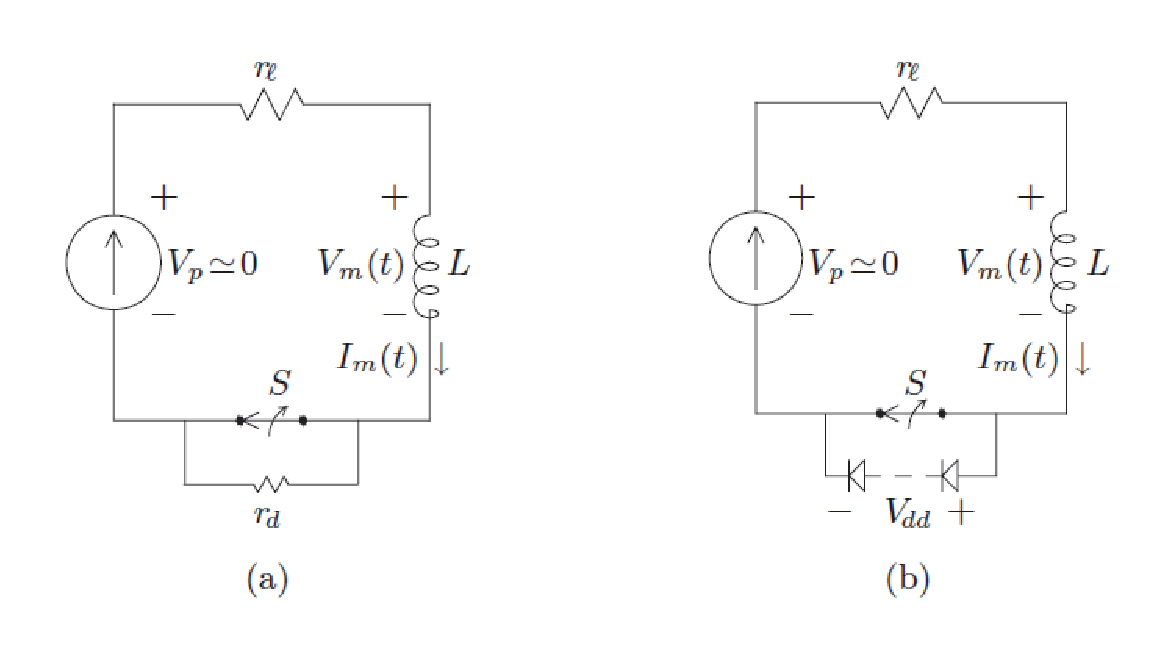
\includegraphics[scale=0.6]{chpt8/figs/fig8.23.eps}
	\caption{Circuits for “slow” discharge modes: (a}
\end{figure}






\begin{equation}% 8.77b
\frac{dI_m(t)}{dt}=-\frac{V_{dd}}{L}
\end{equation}


\subsection{讨论8.3:低阻电阻器设计}
\begin{equation}% 8.78a
r_d=\frac{\rho\ell}{\omega\delta}
\end{equation}
\begin{equation}% 8.78b
r_dI_m(0)^2\simeq 2\omega\ell g_{cv}
\end{equation}
\begin{equation}% 8.79a
\ell\simeq r_dI_m(0)\sqrt{\frac{\delta}{2\rho g_{cv}}}
\end{equation}
\begin{equation}% 8.79b
\omega\simeq I_m(0)\sqrt{\frac{\rho}{2\delta g_{cv}}}
\end{equation}
\begin{equation}% page521 第一个
\ell\simeq(0.01\Omega)(250\ \mathrm{A})\sqrt{\frac{(250\times 10^{-6}\ \mathrm{m})}{2(10^{-6}\ \mathrm{\Omega m})(20\ \mathrm{W/m^2})}} 
\simeq 6.3\ \mathrm{m}
\end{equation}
\begin{equation}% page521 第二个
\omega\simeq(250\ \mathrm{A})\sqrt{\frac{(10^{-6}\ \mathrm{\Omega m})}{2(250\times 10^{-6}\ \mathrm{m})(20\ \mathrm{W/m^2})}} 
\simeq 2.5\ \mathrm{m}
\end{equation}
\begin{equation}% page521第三个
\ell\simeq(0.01\Omega)(250\ \mathrm{A})\sqrt{\frac{(250\times 10^{-6}\ \mathrm{m})}{2(10^{-6}\ \mathrm{\Omega m})(20\times 10^3\ \mathrm{W/m^2})}} 
\simeq 20\ \mathrm{cm}
\end{equation}
\begin{equation}% page521 第四个
\omega\simeq(250\ \mathrm{A})\sqrt{\frac{(10^{-6}\ \mathrm{\Omega m})}{2(250\times 10^{-6}\ \mathrm{m})(20\times 10^3\ \mathrm{W/m^2})}} 
\simeq 8\ \mathrm{cm}
\end{equation}


\subsection{讨论8.4:过热\& 内部电压判据}

\begin{align*}% page522 8.30a
J_{m_{op}}^{sh}&=\left(\frac{1+\gamma_{m/s}}{\gamma_{m/s}}\right)\frac{f_r\pi(\alpha+1)\rho_m(T_f)Z(T_f,T_i)}{2}\sqrt{\frac{a_1}{2\mu_o\ \mathcal{L}(\alpha,\beta)E_m}} \\
&=\left(\frac{1+1}{1}\right)\frac{(0.5)\pi(1.3+1)(1.11\times 10^{-8}\ \mathrm{\Omega m})(10.5\times 10^{16}\ \mathrm{A^2s/m^4})}{2}\times \\
&=\sqrt{\frac{0.15\ \mathrm{m}}{2(4\pi\times 10^{-7}\ \mathrm{H/m})(0.54)(3\times 10^6\ \mathrm{J})}} \\
&\simeq 2(21.1\times 10^8\ \mathrm{J/m^3})(0.19\ \mathrm{Am/J})\\
&\simeq 805\ \mathrm{MA/m^2}=805\ \mathrm{A/mm^2}
\end{align*}



\begin{align*}% 8.40b
J_{m_{op}}^{V}&=\frac{2}{f_r(1-f_r)}\left[\frac{\sqrt{\mathcal{L}(\alpha,\beta)}}{\pi(\alpha+1)}\right]\left[\frac{V_{bk}I_{op}}{\rho_m(T_f)}\sqrt{\frac{2\mu_o}{a_1E_m}}\right] \\
&=\frac{2}{0.5(1-0.5)}\left[\frac{\sqrt{0.54}}{\pi(1.3+1)}\right]\left[\frac{(10^4\ \mathrm{V})(300\ \mathrm{A})}{(1.11\times 10^{-8}\ \mathrm{\Omega m})}\sqrt{\frac{2(4\pi\times 10^{-7}\ \mathrm{H/m})}{(0.15\ \mathrm{m})(3\times 10^6\ \mathrm{J})}}\right] \\
&=8(0.102)(2.70\times 10^{14}\ \mathrm{A^2/m})(2.36\times 10^{-6}\ \mathrm{A^{-1}m^{-1}}) \\
&=5.2\times 10^8\ \mathrm{A/m^2}=520\ \mathrm{A/mm^2}
\end{align*}


\subsection{讨论8.5:Bi2223带电流引线的保护}

\begin{equation}% 8.80
a_mk_m\frac{d^2T}{dz^2}+\frac{\rho_mI_{t}^{2}}{a_m}=0
\end{equation}
\begin{equation}% 8.81
T(\zeta)=T_{cl}+(T_{wm}-T_{cl})\zeta+\frac{\rho_m\ell^2I_{t}^{2}}{2a_{m}^{2}k_m}(\zeta-\zeta^2)
\end{equation}
\begin{equation}% 8.82a
\zeta(T_{pk})=\frac{1}{2}+\frac{a_{m}^{2}k_m}{\rho_mI_{t}^{2}\ell^2}(T_{wm}-T_{cl})
\end{equation}
\begin{equation}% 8.82b
T_{pk}\simeq \frac{1}{2}(T_{cl}+T_{wm})+\frac{\rho_mI_{t}^{2}\ell^2}{8a_{m}^{2}k_m}
\end{equation}
\begin{equation}% page523 最后一个
\frac{a_{m}^{2}k_m}{\rho_mI_{t}^{2}\ell^2}(T_{wm}-T_{cl})=\frac{(8\times 10^{-3}\ \mathrm{cm^2})^2(2\ \mathrm{W/cm K})}{(1\times 10^{-6}\ \mathrm{\Omega cm})(50\ \mathrm{A})^2(15\ \mathrm{cm})^2} 
\simeq 0.01
\end{equation}
\begin{equation}% page524 第一个
T_{pk}\simeq\frac{1}{2}(T_{cl}+\frac{\rho_mI_{t}^{2}\ell^2}{8a_{m}^{2}k_m} 
=\frac{1}{2}(10\ \mathrm{K}+70\ \mathrm{K})+\frac{(1\times 10^{-6}\ \mathrm{\Omega cm})(50\ \mathrm{A})^2(15\ \mathrm{cn})^2}{8(8\times 10^{-3}\ \mathrm{cm^2})^2(2\ \mathrm{W/cm K})}\simeq 590\ \mathrm{K}
\end{equation}



\subsection{讨论8.6:$MgB_2$磁体的主动保护}



\begin{figure}
	\centering
	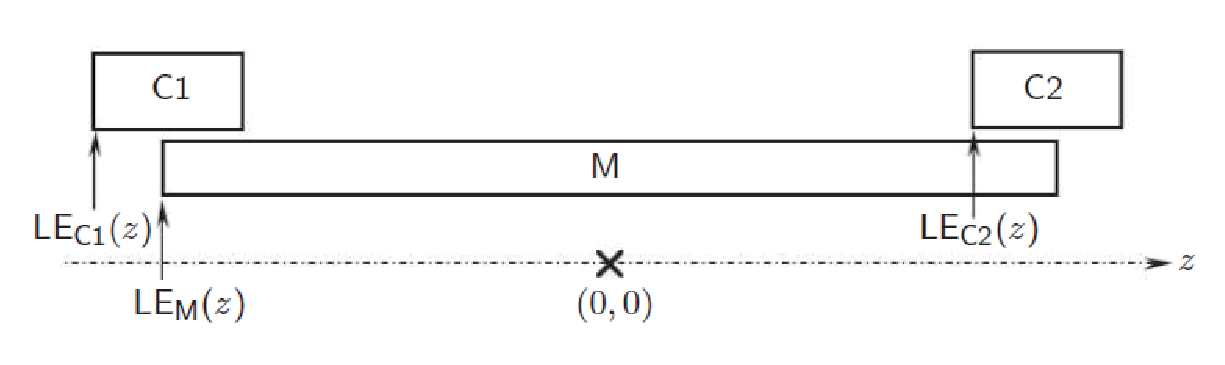
\includegraphics[scale=0.6]{chpt8/figs/fig8.24.eps}
	\caption{Schematic drawing of a magnet comprised of three solenoids}
\end{figure}


\begin{figure}
	\centering
	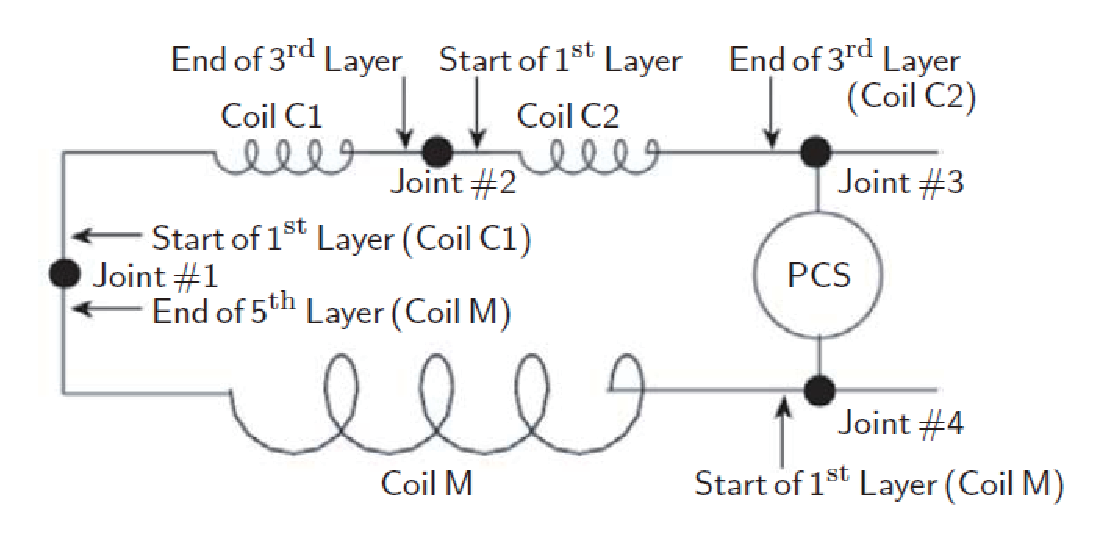
\includegraphics[scale=0.6]{chpt8/figs/fig8.25.eps}
	\caption{Schematic drawing of a 3-coil arrangement, shunted by PCS for persistent}
\end{figure}




\begin{equation}% page528 8.9c
\int_{T_i}^{T_f}\frac{C_m(T)}{\rho_m(T)}dT=\left(\frac{A_m}{A_{cd}}\right)J_{m_o}^{2}\tau_{ah}
\end{equation}
\begin{equation}% page528 6.33
R_{mz}=\sqrt{\frac{3k_{wd}(T_c-T_{op})}{\rho_mJ_{m}^{2}}}
\end{equation}
\begin{equation}% 8.83a
V_M(t)=V_r(t)+(L_M+M_{MC1}+M_{MC2})\frac{dI_{op}(t)}{dt}
\end{equation}
\begin{equation}% 8.83b
V_{C1}(t)=(L_{C1}+M_{C1M}+M_{C1C2})\frac{dI_{op}}{dt}=V_{C2}(t)=-\frac{1}{2}V_M(t)
\end{equation}
\begin{equation}% 8.83c
V_M(t)+V_{C1}(t)+V_{C2}(t)=0
\end{equation}



\subsection{问题8.6:NMR磁体的被动保护}


\begin{figure}
	\centering
	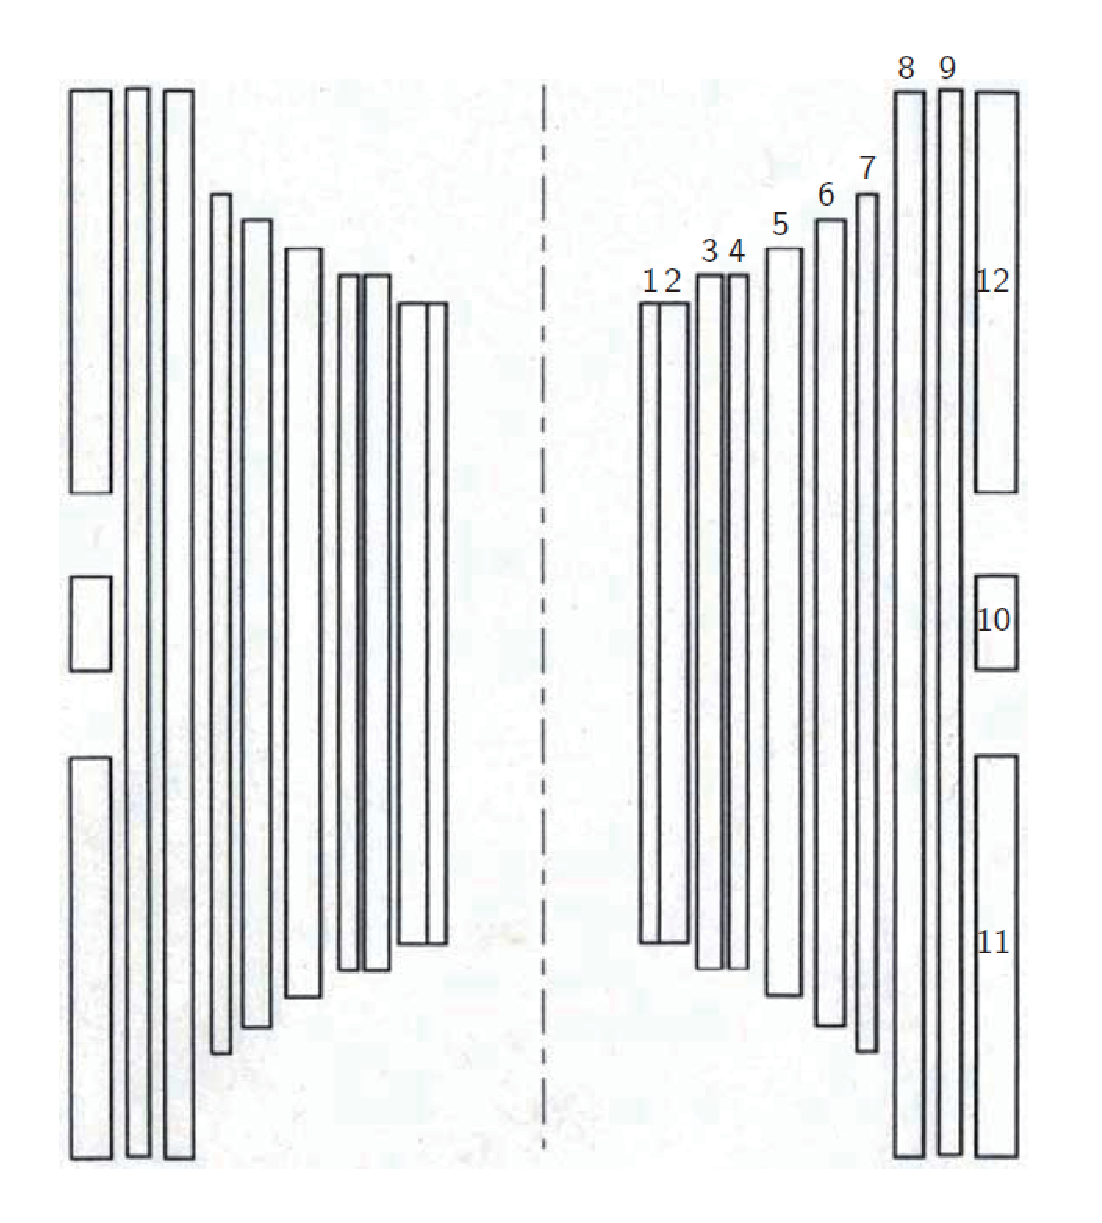
\includegraphics[scale=0.6]{chpt8/figs/fig8.26.eps}
	\caption{Drawing showing the locations of 12 coils in }
\end{figure}


\begin{figure}
	\centering
	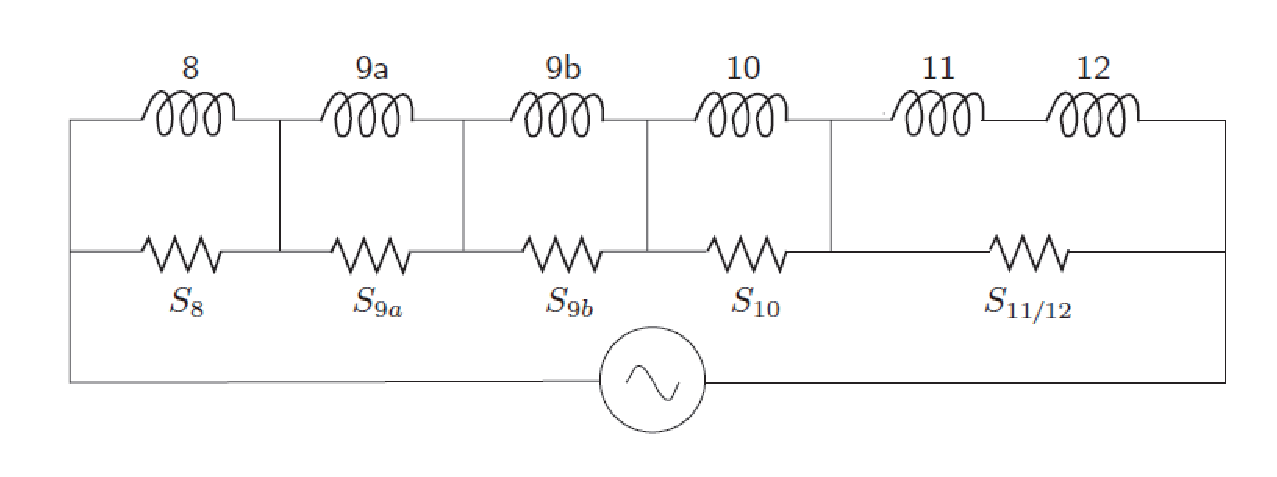
\includegraphics[scale=0.6]{chpt8/figs/fig8.27.eps}
	\caption{Circuit for the NbTi coils}
\end{figure}


\begin{figure}
	\centering
	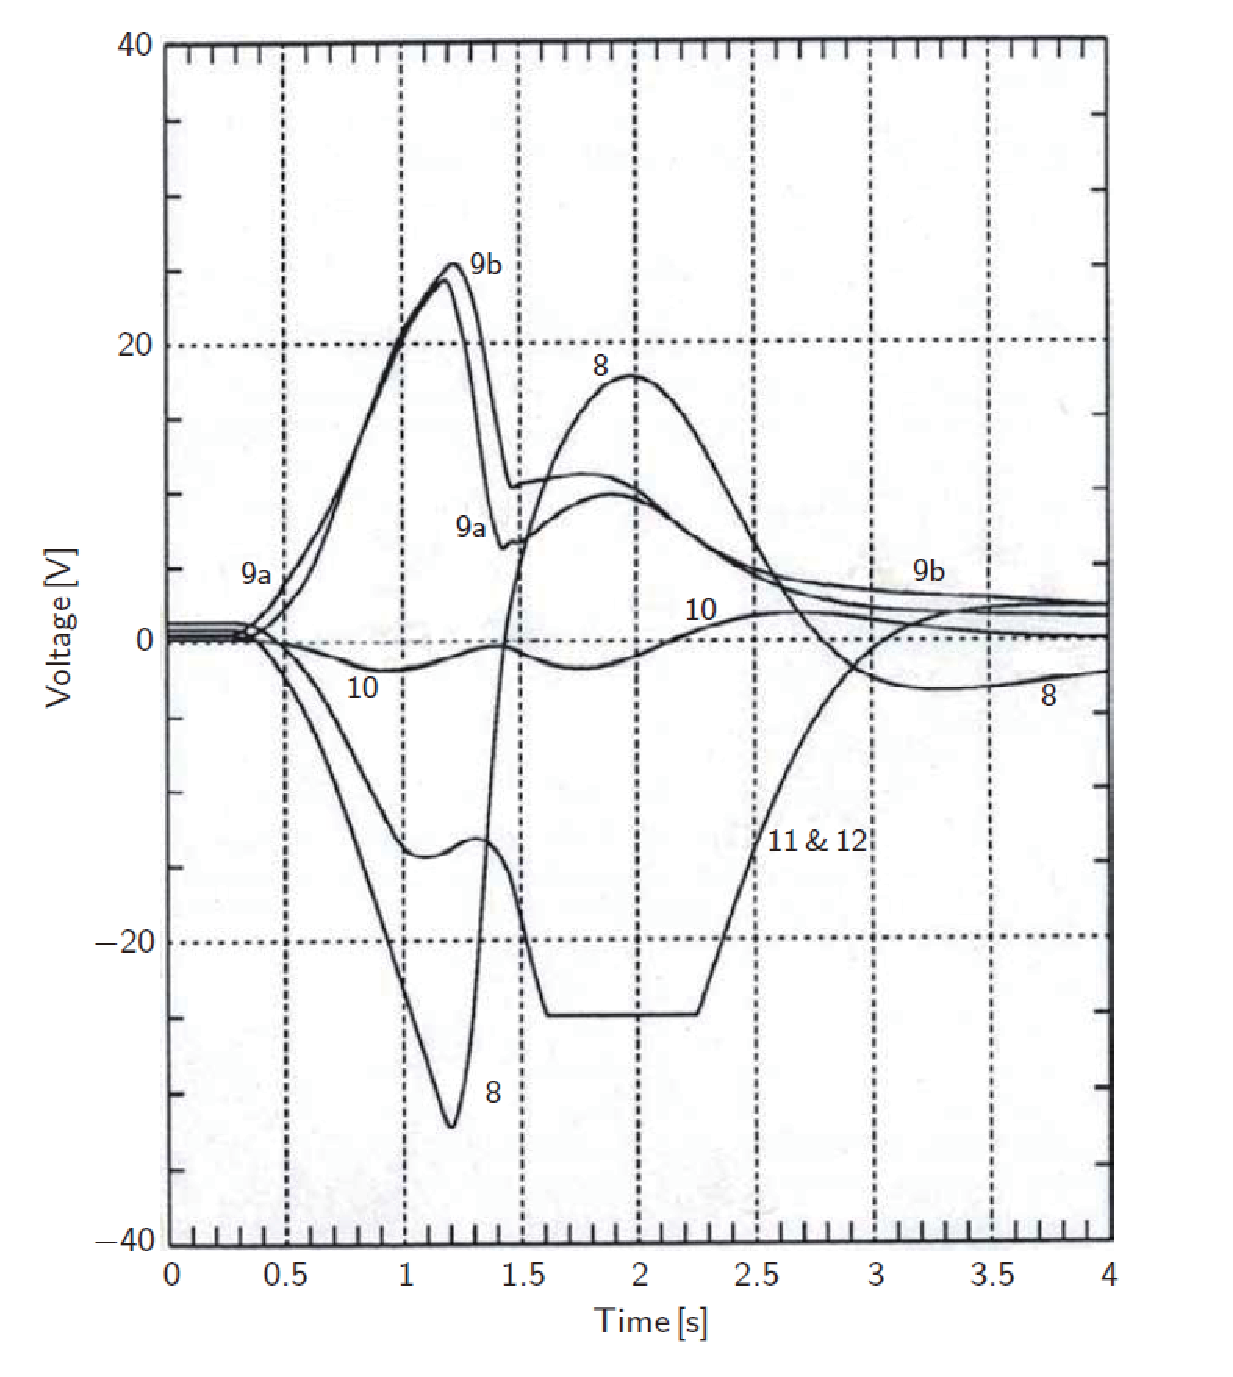
\includegraphics[scale=0.6]{chpt8/figs/fig8.28.eps}
	\caption{Voltage traces recorded acro}
\end{figure}


\begin{figure}
	\centering
	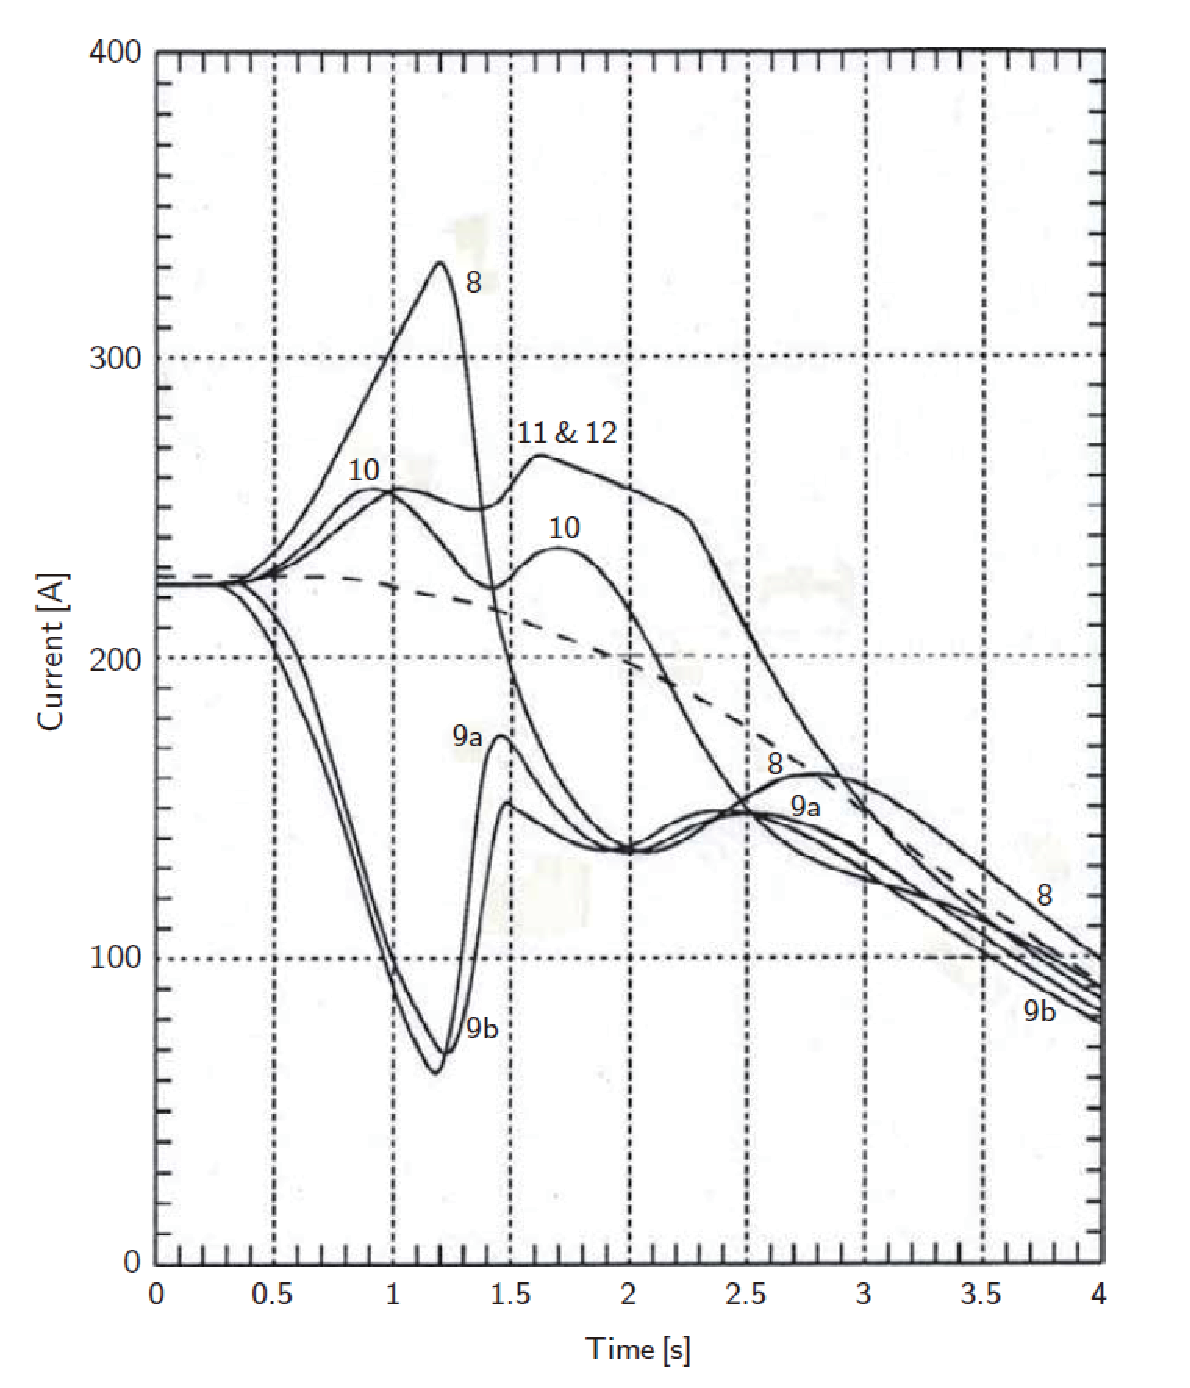
\includegraphics[scale=0.6]{chpt8/figs/fig8.29.eps}
	\caption{Current traces through Coils 8, 9a, 9b, 10, and 11/12 corresponding}
\end{figure}



\begin{equation}% 8.84a
I_8=I_0-\frac{V_8}{S_8}
\end{equation}
\begin{equation}% 8.84b
I_{9a}=I_0-\frac{V_{9a}}{S_{9a}}
\end{equation}
\begin{equation}% 8.84c
I_{9b}=I_0-\frac{V_{9b}}{S_{9b}}
\end{equation}
\begin{equation}% 8.84d
I_{10}=I_0-\frac{V_{10}}{S_{10}}
\end{equation}
\begin{equation}% 8.84e
I_{11/12}=I_0\frac{V_{11/12}}{S_{11/12}}
\end{equation}


\subsubsection{问题8.6之解}

\begin{equation}% page535 8.84a
I_8=I_0-I_{r8}  
=I_0-\frac{V_8}{S_8}
\end{equation}
\begin{equation}% page535 8.84b
I_{9a}=I_8+I_{r8}-I_{r9a}=I_0-\frac{V_8}{S_8}+\frac{V_8}{S_8}-\frac{V_{9a}}{S_{9a}}
=I_0-\frac{V_{9a}}{S_{9a}}
\end{equation}
\begin{equation}% page535 8.84c
I_{9b}=I_{9a}+\frac{V_{9a}}{S_{9a}}-\frac{V_{9b}}{S_{9b}}=I_0-\frac{V_{9a}}{S_{9a}}+\frac{V_{9a}}{S_{9a}}-\frac{V_{9b}}{S_{9b}} 
=I_0\frac{V_{9b}}{S_{9b}}
\end{equation}
\begin{equation}% page535 8.84d
I_{10}=I_{9b}+\frac{V_{9b}}{S_{9b}}-\frac{V_{10}}{S_{10}}=I_0-\frac{V_{9b}}{S_{9b}}+\frac{V_{9b}}{S_{9b}}-\frac{V_{10}}{S_{10}}
=I_0-\frac{V_{10}}{S_{10}}
\end{equation}
\begin{equation}% page535 8.84e
I_{11/12}=I_{10}+\frac{V_{10}}{S_{10}}-\frac{V_{11/12}}{S_{11/12}}=I_0-\frac{V_{10}}{S_{10}}+\frac{V_{10}}{S_{10}}-\frac{V_{11/12}}{S_{11/12}}
=I_0-\frac{V_{11/12}}{S_{11/12}}
\end{equation}
\begin{equation}% page535 S6.1
V_8=V_r\mid_8+L_8\frac{dI_8}{dt}+M_{8,9a}\frac{dI_{9a}}{dt}+M_{8,9b}\frac{dI_{9b}}{dt} 
+M_{8,10}\frac{dI_{10}}{dt}+M_{8,11}\frac{dI_{11}}{dt}+M_{8,12}\frac{dI_{12}}{dt}
\end{equation}
\begin{equation}% page535 S6.2a
V_8\simeq V_r\mid_8+(4.413\ \mathrm{H})(84.5\ \mathrm{A/s})+(2.268\ \mathrm{H})(-154.1\ \mathrm{A/s}) 
+(2.243\ \mathrm{H})(-107.1\ \mathrm{A/s})+(0.715\ \mathrm{H})(41.3\ \mathrm{A/s}) 
+(2.747\ \mathrm{H})(33.6\ \mathrm{A/s})+(2.755\ \mathrm{H})(33.6\ \mathrm{A/s})
\end{equation}
\begin{equation}% page535 S6.2b
V_8=V_r\mid_8+372.9-349.5-240.2+39.4+92.4+92.6 
=V_r\mid_8-2.5\ \mathrm{V}
\end{equation}
\begin{equation}% page536 S6.3a
V_8=V_r\mid_8+(4.413\ \mathrm{H})(147.2\ \mathrm{A/s})+(2.268\ \mathrm{H})(-234.7\ \mathrm{A/s}) 
+(2.243\ \mathrm{H})(-198.1\ \mathrm{A/s})+(0.715\ \mathrm{H})(-44.8\ \mathrm{A/s}) 
+(2.747\ \mathrm{H})(19.3\ \mathrm{A/s})+(2.755\ \mathrm{H})(19.3\ \mathrm{A/s})
\end{equation}
\begin{equation}% page536 S6.3b
V_8=V_r\mid_8+(649.6-532.3-444.3-32.0+53.0+53.2)[\mathrm{V}]
=V_r\mid_8-252.9[\mathrm{V}]
\end{equation}
\begin{equation}% page536 S6.4
P_{mg}=\sum_{n=8}^{12}V_r\mid_n\times I_n
\end{equation}
\begin{equation}% page536 S6.5
P_{mg}\simeq\left(\tilde{V}-\sum_{m,n=8}^{12}L_{m,n}\frac{d\tilde{I}}{dt}\right)\times \tilde{I}
\end{equation}
\begin{equation}% page536 S6.6
P_{mg}\simeq[0-(60.25\ \mathrm{H})(-50\ \mathrm{A/s})](90\ \mathrm{A})\simeq 270,000\ \mathrm{W}
\end{equation}




\subsection{讨论8.7:HTS磁体到底要不要保护?}
\begin{equation}% 8.85a
\$_{T/w}=\$_M+\$_{qp}
\end{equation}
\begin{equation}% 8.85b
\$_{T/wo}=\$_M+P_{dm}(\$_M+\$_{ra})
\end{equation}